\documentclass{wissdoc}
% Autor: Roland Bless 1996-2009, bless <at> kit.edu
% ----------------------------------------------------------------
% Diplomarbeit - Hauptdokument
% ----------------------------------------------------------------
%%
%% $Id: thesis.tex 65 2012-05-10 10:32:11Z bless $
%%
%
% Zum Erstellen zweiseitiger PDFs (für Buchdruck) in der Datei "wissdoc.cls" folgende Zeile abändern:
%
% \LoadClass[a4paper,12pt,oneside]{book} % diese Klasse basiert auf ``book''
% in
%\LoadClass[a4paper,12pt,titlepage]{book} % diese Klasse basiert auf ``book''
%
%
% wissdoc Optionen: draft, relaxed, pdf --> siehe wissdoc.cls
% ------------------------------------------------------------------
% Weitere packages: (Dokumentation dazu durch "latex <package>.dtx")
\usepackage[numbers,sort&compress]{natbib}
% \usepackage{varioref}
% \usepackage{verbatim}
% \usepackage{float}    %z.B. \floatstyle{ruled}\restylefloat{figure}
% \usepackage{subfigure}
% \usepackage{fancybox} % für schattierte,ovale Boxen etc.
% \usepackage{tabularx} % automatische Spaltenbreite
% \usepackage{supertab} % mehrseitige Tabellen
% \usepackage[svnon,svnfoot]{svnver} % SVN Versionsinformation 
%% ---------------- end of usepackages -------------

%\svnversion{$Id: thesis.tex 65 2012-05-10 10:32:11Z bless $} % In case that you want to include version information in the footer

%% Informationen für die PDF-Datei
\hypersetup{
 pdfauthor={Benedikt Lüken-Winkels},
 pdftitle={Bachelorarbeit_1138844_s4beluek}
 pdfsubject={Graphreduktionsregeln},
 pdfkeywords={Graphreduktionsregeln, Knotenüberdeckung, Bachelorarbeit}
}

% Macros, nicht unbedingt notwendig
%%%%%%%%%%%%%%%%%%%%%%%%%%%%%%%%%%%%%%%%%%%%%%%%%%%%%%%%%%
% macros.tex -- einige mehr oder weniger nuetzliche Makros
% Autor: Roland Bless 1998
%%%%%%%%%%%%%%%%%%%%%%%%%%%%%%%%%%%%%%%%%%%%%%%%%%%%%%%%%%
% $Id: macros.tex 33 2007-01-23 09:00:59Z bless $
%%%%%%%%%%%%%%%%%%%%%%%%%%%%%%%%%%%%%%%%%%%%%%%%%%%%%%%%%%


%%%%%%%%%%%%%%%%%%%%%%%
% Kommentare 
%%%%%%%%%%%%%%%%%%%%%%%
\ifnotdraftelse{
\newcommand{\Kommentar}[1]{}
}{\newcommand{\Kommentar}[1]{{\em #1}}}
% Alles innerhalb von \Hide{} oder \ignore{} 
% wird von LaTeX komplett ignoriert (wie ein Kommentar)
\newcommand{\Hide}[1]{}
\let\ignore\Hide

%%%%%%%%%%%%%%%%%%%%%%%%%
% Leere Seite ohne Seitennummer, wird aber gezaehlt
%%%%%%%%%%%%%%%%%%%%%%%%%

\newcommand{\leereseite}{% Leerseite ohne Seitennummer, nächste Seite rechts (wenn 2-seitig)
 \clearpage{\pagestyle{empty}\cleardoublepage}
}
%%%%%%%%%%%%%%%%%%%%%%%%%%
% Flattersatz rechts und Silbentrennung, Leerraum nach rechts maximal 1cm
%%%%%%%%%%%%%%%%%%%%%%%%%%
\makeatletter
\newcommand{\myraggedright}{%
 \let\\\@centercr\@rightskip 0pt plus 1cm
 \rightskip\@rightskip
  \leftskip\z@skip
  \parindent\z@
  \spaceskip=.3333em
  \xspaceskip=.5em}
\makeatother

\makeatletter
\newcommand{\mynewline}{%
 \@centercr\@rightskip 0pt plus 1cm
}
\makeatother


%%%%%%%%%%%%%%%%%%%%%%%%%%
% Für Index
%%%%%%%%%%%%%%%%%%%%%%%%%%
\makeatletter
\def\mydotfill{\leavevmode\xleaders\hb@xt@ .44em{\hss.\hss}\hfill\kern\z@}
\makeatother
\def\bold#1{{\bfseries #1}}
\newbox\dbox \setbox\dbox=\hbox to .4em{\hss.\hss} % dot box for leaders
\newskip\rrskipb \rrskipb=.5em plus3em % ragged right space before break
\newskip\rrskipa \rrskipa=-.17em plus -3em minus.11em % ditto, after
\newskip\rlskipa \rlskipa=0pt plus3em % ragged left space after break
\newskip\rlskipb \rlskipb=.33em plus-3em minus.11em % ragged left before break
\newskip\lskip \lskip=3.3\wd\dbox plus1fil minus.3\wd\dbox % for leaders
\newskip \lskipa \lskipa=-2.67em plus -3em minus.11em %after leaders
\mathchardef\rlpen=1000 \mathchardef\leadpen=600
\def\rrspace{\nobreak\hskip\rrskipb\penalty0\hskip\rrskipa}
\def\rlspace{\penalty\rlpen\hskip\rlskipb\vadjust{}\nobreak\hskip\rlskipa}
\let\indexbreak\rlspace
\def\raggedurl{\penalty10000 \hskip.5em plus15em \penalty0 \hskip-.17em plus-15em minus.11em}
\def\raggeditems{\nobreak\hskip\rrskipb \penalty\leadpen \hskip\rrskipa %
\vadjust{}\nobreak\leaders\copy\dbox\hskip\lskip %
\kern3em \penalty\leadpen \hskip\lskipa %
\vadjust{}\nobreak\hskip\rlskipa}
\renewcommand*\see[2]{\rlspace\emph{\seename}~#1} % from makeidx.sty

%%%%%%%%%%%%%%%%%%%%%%%%%%
% Neue Seite rechts, leere linke Seite ohne Headings
%%%%%%%%%%%%%%%%%%%%%%%%%%
\newcommand{\xcleardoublepage}
{{\pagestyle{empty}\cleardoublepage}}

%%%%%%%%%%%%%%%%%%%%%%%%%%
% Tabellenspaltentypen (benoetigt colortbl)
%%%%%%%%%%%%%%%%%%%%%%%%%%
\newcommand{\PBS}[1]{\let\temp=\\#1\let\\=\temp}
\newcolumntype{y}{>{\PBS{\raggedright\hspace{0pt}}}p{1.35cm}}
\newcolumntype{z}{>{\PBS{\raggedright\hspace{0pt}}}p{2.5cm}}
\newcolumntype{q}{>{\PBS{\raggedright\hspace{0pt}}}p{6.5cm}}
\newcolumntype{g}{>{\columncolor[gray]{0.8}}c} % Grau
\newcolumntype{G}{>{\columncolor[gray]{0.9}}c} % helleres Grau

%%%%%%%%%%%%%%%%%%%%%%%%%%
% Anführungszeichen oben und unten
%%%%%%%%%%%%%%%%%%%%%%%%%%
\newcommand{\anf}[1]{"`{#1}"'}

%%%%%%%%%%%%%%%%%%%%%%%%%%
% Tiefstellen von Text
%%%%%%%%%%%%%%%%%%%%%%%%%%
% S\tl{0} setzt die 0 unter das S (ohne Mathemodus!)
% zum Hochstellen gibt es uebrigens \textsuperscript
\makeatletter
\DeclareRobustCommand*\textlowerscript[1]{%
  \@textlowerscript{\selectfont#1}}
\def\@textlowerscript#1{%
  {\m@th\ensuremath{_{\mbox{\fontsize\sf@size\z@#1}}}}}
\let\tl\textlowerscript
\let\ts\textsuperscript
\makeatother

%%%%%%%%%%%%%%%%%%%%%%%%%%
% Gauß-Klammern
%%%%%%%%%%%%%%%%%%%%%%%%%%
\newcommand{\ceil}[1]{\lceil{#1}\rceil}
\newcommand{\floor}[1]{\lfloor{#1}\rfloor}

%%%%%%%%%%%%%%%%%%%%%%%%%%
% Average Operator (analog zu min, max)
%%%%%%%%%%%%%%%%%%%%%%%%%%
\def\avg{\mathop{\mathgroup\symoperators avg}}

%%%%%%%%%%%%%%%%%%%%%%%%%%
% Wortabkürzungen
%%%%%%%%%%%%%%%%%%%%%%%%%%
\def\zB{z.\,B.\ }
\def\dh{d.\,h.\ }
\def\ua{u.\,a.\ }
\def\su{s.\,u.\ }
\newcommand{\bzw}{bzw.\ }

%%%%%%%%%%%%%%%%%%%%%%%%%%%%%%%%%%%
% Einbinden von Graphiken
%%%%%%%%%%%%%%%%%%%%%%%%%%%%%%%%%%%
% global scaling factor
\def\gsf{0.9}
%% Graphik, 
%% 3 Argumente: Datei, Label, Unterschrift
\newcommand{\Abbildung}[3]{%
\begin{figure}[tbh] %
\centerline{\scalebox{\gsf}{\includegraphics*{#1}}} %
\caption{#3} %
\label{#2} %
\end{figure} %
}
\let\Abb\Abbildung
%% Abbps
%% Graphik, skaliert, Angabe der Position
%% 5 Argumente: Position, Breite (0 bis 1.0), Datei, Label, Unterschrift
\newcommand{\Abbildungps}[5]{%
\begin{figure}[#1]%
\begin{center}
\scalebox{\gsf}{\includegraphics*[width=#2\textwidth]{#3}}%
\caption{#5}%
\label{#4}%
\end{center}
\end{figure}%
}
\let\Abbps\Abbildungps
%% Graphik, Angabe der Position, frei wählbares Argument für includegraphics
%% 5 Argumente: Position, Optionen, Datei, Label, Unterschrift
\newcommand{\Abbildungpf}[5]{%
\begin{figure}[#1]%
\begin{center}
\scalebox{\gsf}{\includegraphics*[#2]{#3}}%
\caption{#5}%
\label{#4}%
\end{center}
\end{figure}%
}
\let\Abbpf\Abbildungpf

%%
% Anmerkung: \resizebox{x}{y}{box} skaliert die box auf Breite x und Höhe y,
%            ist x oder y ein !, dann wird das usprüngliche 
%            Seitenverhältnis beibehalten.
%            \rescalebox funktioniert ähnlich, nur das dort ein Faktor
%            statt einer Dimension angegeben wird.
%%
% \Abbps{Position}{Breite in Bruchteilen der Textbreite}{Dateiname}{Label}{Bildunterschrift}
%

\newcommand{\refAbb}[1]{%
s.~Abbildung \ref{#1}}

%%%%%%%%%%%%%%%%%%%%
%% end of macros.tex
%%%%%%%%%%%%%%%%%%%%

% Print URLs not in Typewriter Font
\def\UrlFont{\rm}

\newcommand{\blankpage}{% Leerseite ohne Seitennummer, nächste Seite rechts
 \clearpage{\pagestyle{empty}\cleardoublepage}
}

%% Einstellungen für das gesamte Dokument

% Trennhilfen
% Wichtig! 
% Im ngerman-paket sind zusätzlich folgende Trennhinweise enthalten:
% "- = zusätzliche Trennstelle
% "| = Vermeidung von Ligaturen und mögliche Trennung (bsp: Schaf"|fell)
% "~ = Bindestrich an dem keine Trennung erlaubt ist (bsp: bergauf und "~ab)
% "= = Bindestrich bei dem Worte vor und dahinter getrennt werden dürfen
% "" = Trennstelle ohne Erzeugung eines Trennstrichs (bsp: und/""oder)

% Trennhinweise fuer Woerter hier beschreiben
\hyphenation{
% Pro-to-koll-in-stan-zen
Kno-ten-ü-ber-deck-ung
Kno-ten-ü-ber-deck-ungs-pro-blem
Re-duk-tions-re-geln
Graph-re-duk-tions-re-geln
Graph-re-duk-tion
}

% Index-Datei öffnen
\ifnotdraft{\makeindex}

\begin{document}

\frontmatter
\pagenumbering{roman}
\ifnotdraft{
 %% Titelseite
%% Vorlage $Id: titelseite.tex 61 2012-05-03 13:58:03Z bless $

\def\usesf{}
\let\usesf\sffamily % diese Zeile auskommentieren für normalen TeX Font

\newsavebox{\Erstgutachter}
\savebox{\Erstgutachter}{\usesf Prof.~Dr.~Henning~Fernau}
\newsavebox{\Zweitgutachter}
\savebox{\Zweitgutachter}{\usesf  Prof.~Dr.~Stefan~Näher}
\newsavebox{\Betreuer}
\savebox{\Betreuer}{\usesf Prof.~Dr.~Henning~Fernau}

\begin{titlepage}
\setlength{\unitlength}{1pt}
\begin{picture}(0,0)(85,770)
%\includegraphics[width=\paperwidth]{logos/KIT_Deckblatt}
\end{picture}

\thispagestyle{empty}

%\begin{titlepage}
%%\let\footnotesize\small \let\footnoterule\relax
\begin{center}
\hbox{}
\vfill
{\usesf
{\huge\bfseries Untersuchung von Graphreduktionsregeln beim Knotenüberdeckungsproblem\par}
\vskip 1.8cm
{\huge Bachelorarbeit}\\
\vskip 0.5cm
zur Erlangung des akademischen Grades\\
Bachelor (B.Sc.) 
\vskip 1.5cm

{\large Universität Trier\\
FB IV - Informatikwissenschaften\\
Lehrstuhl für theoretische Informatik\\}

\vskip 3cm
\begin{tabular}{p{3.5cm}l}
Gutachter: & \usebox{\Erstgutachter} \\
 & \usebox{\Zweitgutachter} \\
Betreuer: & \usebox{\Betreuer} \\
\end{tabular}
\vskip 3cm
Vorgelegt am xx.xx.xxxx von:\\
\vskip .5cm
Benedikt Lüken-Winkels\\
Bahnhofstraße 32\\
54292 Trier\\
s4beluek@uni-trier.de\\
Matr.-Nr. 1138844


}
\end{center}
\vfill
\end{titlepage}
%% Titelseite Ende


%%% Local Variables: 
%%% mode: latex
%%% TeX-master: "thesis"
%%% End: 

 %\blankpage % Leerseite auf Titelrückseite
 \chapter*{Zusammenfassung}
%% ==============================
Gegenstand dieser Arbeit ist der Vergleich und die Anwendung von Graphreduktionsregeln für das Knotenüberdeckungsproblem. Die Regeln als solche, das Verhalten verschiedener Regeln in der Praxis und der Effekt von deren kombinierter Anwendung wurden untesucht. Umsetzung und Implementierung der Algorithmen geschah in der Programmiersprache \emph{C++} mithilfe der \emph{C++}-Library LEDA. Es stellte sich heraus, dass das Ergebnis der Reduktion in hohem Maße sowohl von der jeweiligen Kombination, als auch der Reihenfolge, in der die Reduktionsregeln an einem Problemgraphen angewandt werden, abhängt. Zudem wurde eine Konfiguration für die hier implementierte Kronenregel gefunden, welche die Reduktion der Regel in der Praxis deutlich verbessert. Die Abhängigkeit der Regel von dieser Einstellung wurde bereits durch andere Untersuchungen zum Thema entdeckt \cite{paper:7}. Die besten Ergebnisse bei der Reduktion pro Graph am eigens erstellten Testset erreichte die Anwendung in der Reihenfolge Nemhauser-Trotter-Regel - Kronenregel - Grad$_{1}$-Regel. Hier zeigten sich einige besondere Graphen, welche sich im Vergleich zu den anderen Graphen aus der gleichen Kategorie, beziehungsweise mit der gleichen Kantenanzahl, untypisch verhalten haben. 
}
%
%% *************** Hier geht's ab ****************
%% ++++++++++++++++++++++++++++++++++++++++++
%% Verzeichnisse
%% ++++++++++++++++++++++++++++++++++++++++++
\ifnotdraft{
{\parskip 0pt\tableofcontents} % toc bitte einzeilig
%\blankpage
\listoffigures
%\blankpage
\listoftables
%\blankpage
}


%% ++++++++++++++++++++++++++++++++++++++++++
%% Hauptteil
%% ++++++++++++++++++++++++++++++++++++++++++
\graphicspath{{img/}}

\mainmatter
\pagenumbering{arabic}
%% Einleitung.tex
%% $Id: einleitung.tex 61 2012-05-03 13:58:03Z bless $
%%

\chapter{Einleitung}
\label{ch:Einleitung}
%% ==============================
Die Einleitung besteht aus der Motivation, der Problemstellung, der Zielsetzung und einem erster Überblick über den Aufbau der Arbeit.

%% ==============================
\section{Motivation}
%% ==============================
\label{ch:Einleitung:sec:Motivation}
Das \emph{Knotenüberdeckungsproblem}, oder englisch Vertex Cover, ist ein nachgewiesen NP-vollständiges Problem \cite{intract}, kann also von einem nichtdeterministischen Algorithmus in Polinomialzeit gelöst werden. Um das Problem zu erklären, betrachten wir ein Netz von Haushalten, bei dem wir die Möglichkeit haben, in jedem Haushalt einen Stromgenerator zu platzieren, sodass durch alle mit diesem Haus verbundenen Leitungen Strom fließt. Ziel ist, ein stabiles Stromnetz zu schaffen, bei dem jede Leitung an mindestens eine Stromquelle angeschlossen ist. Nun ergibt sich das Problem, dass die Kosten für Stromgeneratoren erheblich sind und daher nur maximal \emph{k} Geräte angeschafft werden können. Es gilt also, aus den \emph{n} Häusern \emph{k} oder weniger auszuwählen, sodass jede Leitung von einem der Häuser in der Auswahl versorgt wird.
\begin{figure}[htb]
\centering
  	{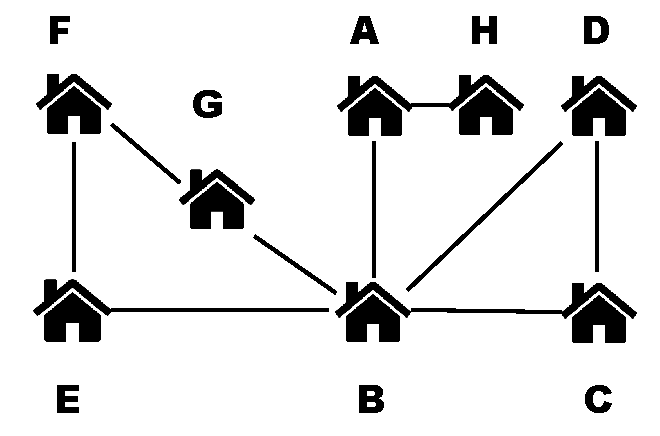
\includegraphics[width=.5\textwidth]{vertexcoverBsp.pdf}}
	\caption{Graph eines Stromnetzes \label{fig:vc}}
\centering
\end{figure}
In Abbildung \ref{fig:vc}\footnote{Icons in der Graphik von https://www.flaticon.com/}   sieht man ein Beispiel für eine solche Probleminstanz. Die Haushalte sind jeweils mit einem Buchstaben gekennzeichnet; jede Linie, beziehungsweise Kante eine Leitung zum Nachbarhaus. Hier ist es möglich eine Lösung für \emph{k} = 4 zu finden, also 4 Häuser mit Generatoren auszustatten, sodass alle Leitungen versorgt sind. Bei einem kleinen Beispiel, wie hier ist zum Beispiel durch ausprobieren leicht zu sehen, dass es keine Lösung mit weniger Häusern, beziehungsweise Generatoren gibt. Um 4 Häuser, die das Problem lösen zu finden, könnten alle Möglichkeiten ausprobiert werden. Ein solcher naiver Algorithmus würde eine Laufzeit von $O(n^{k} \cdot m)$ ($m$ = Anzahl der Leitungen) brauchen, da für jede $k$ große Kombination aus Häusern, die Versorgung der Leitungen überprüft werden muss.\\
Mit einem einfachen Suchbaumalgorithmus betrachtet man jede Leitung nur einmal und entscheidet, welches der beiden Häuser mit einem Generator versorgt werden soll, da mindestens eins der beiden Häuser in der Lösungsmenge ist. Dadurch ergibt sich für jede Entscheindung eine Verzweigung. Nach $k$ Verzweigungen sind dann $k$ Generatoren verteilt und es muss überprüft werden, ob jede Leitung versorgt ist, was wiederum in $m$ Schritten gemacht werden kann. Es ergibt sich eine Laufzeit von $O(2^{k}) \cdot m$.
Nach der Verwendung eines dieser Algroithmen, finden sich die Lösung, dass wenn die Haushalte F, B, A und C oder F, B, A und D mit einem Generator ausgestattet werden, durch alle Leitungen Strom fließt. Für eine Problemgröße wie sie hier geschildert wird, bieten diese Mehtoden eine Lösung. Für eine Häusermenge \emph{n} = 2000 mit entsprechend vielen Leitungen bedeutet das ungefähr $1.148 \cdot 10^{602}$ mögliche Kombinationen.

Es ist leicht zu sehen, dass sich das Stromnetzproblem, ersetzt man die Häuser durch Knoten eines Graphen und die Leitungen durch dessen Kanten, zum Knotenüberdeckungsproblem transformieren lässt. Zu diesem Problem lassen sich zwei Fragestellungen unterscheiden: Zum Einen das Finden einer minimalen Knotenüberdeckung \cite{trees}:
\begin{align*}
EINGABE: &\ Graph\ G=(V,E),\ positive\ Integer\ k\leq |V|\\
AUSGABE: &\ S\subseteq V\ mit\ |S|\leq k,\\
&\ sodass\ jede\ Kante\ aus\ E\ einen\ Endpunkt\ in\ S\ hat.
\end{align*}
Zum Anderen das Entscheidungsproblem, ob es eine Knotenüberdeckung einer Größe $\leq k$ gibt:
\begin{align*}
EINGABE: &\ Graph\ G=(V,E),\ positive\ Integer\ k\leq |V|\\
AUSGABE: &\textit{ Existiert ein}\ S\subseteq V\ mit\ |S|\leq k,\\
&\ sodass\ jede\ Kante\ aus\ E\ einen\ Endpunkt\ in\ S\ hat?
\end{align*}
Letzteres ist in der Liste von Karps 21 NP-vollständigen Problemen zu finden \cite{karp}.
Es existieren weitere reale Probleme, für die das Knotenüberdeckungsproblem anwendbar ist. Abu-Khzam et al \cite{paper:3} schlagen eine Anwendung in der Bioinformatik vor.
Ein nichtdeterministischer Algorithmus kann jede vermeintliche Lösungskombination aus Knoten, beziehzungsweise Haushalten in Polynomialzeit testen \cite{intract}, da lediglich überprüft werden muss, ob die Größe der Lösungsmenge den Wert von \emph{k} überschreitet und ob alle Kanten abgedeckt (Leitungen versorgt) sind.
 Allerdings würde ein naiver Algrithmus für große Eingaben in der Realität nicht in absehbarer Zeit terminieren, wie beispielhaft in Tabelle \ref{tab:exponential} zu sehen ist.
 
 \begin{table}[htb]
\caption{Exponentielle Laufzeit \label{tab:exponential}}
\vspace*{1em}
\centering

\bgroup
\def\arraystretch{1.3}%  1 is the default, change whatever you need

\begin{threeparttable}

\begin{tabular}[c]{l l}
	\hline
	\multicolumn{1}{c}{\textbf{Eingabegröße}} & 
	\multicolumn{1}{c}{\textbf{Laufzeit}} \\ 
	
	\hline

	$2^{1}$& 0.00002s\\
	$2^{10}$& 0.02s\\
	$2^{100}$& ca. $ 2 \cdot 10^{14} $ Jahrtausende \\
	\hline
\end{tabular}

\begin{tablenotes}\footnotesize
\item Beispiel für die Laufzeit einen Algorithmus' mit eine Laufzeit von $O(2^{n})$
\end{tablenotes}

\end{threeparttable}

\egroup

\end{table}
Es ist also sinnvoll, die Eingabe möglichst klein zu halten und zu \emph{reduzieren}, indem einfache Teile des Graphen durch Vorverarbeitung, englisch \emph{Preprocessing}, entfernt werden und gegebenenfalls in die Lösungsmenge aufgenommen werden, Die sollte in Polinomialzeit geschehen, um die gesamte Laufzeit zu reduzieren. Das Ziel der in dieser Arbeit verwendeten Reduktionsregeln ist für einen gegebenen Graphen $G=(V,E)$ und einer natürlichen Zahl $k$ und der Problemstellung $VC(G,k)$ das Finden und Entfernen eines induzierten Teilgraphen $G' \subseteq G$ und Verkleinerung von $k$
sodass für den Problemkern $G'' = G \setminus G'$ gilt, dass $VC(G,k) = VC(G'',k'') \cup C\ mit\ C=VC(G', k'')$, wobei $C=VC(G', k'')$ in Polinomialzeit durch die Regeln berechnen lässt. Für den Suchbaumalgorithmus (mit $O(2^{k} \cdot m)$) bedeutet jede Reduzierung von $k$ eine Verdoppelung der Geschwindigkeit. 


%% ==============================
\section{Problemstellung}
%% ==============================
\label{ch:Einleitung:sec:Problemstellung}

Das Knotenüberdeckungsproblem ist in der Literatur viel vertreten und es wurden verschiedene Reduktionsregeln entdeckt. In dieser Arbeit werden einfachere Reduktionsregeln, genauer gesagt die Grad$_{0}$-, Grad$_{1}$- und Buss-Regel betrachtet, als auch Nemhauser-Trotter-Regel und Kronenregel, welche sich weitaus komplexer gestalten. Jede Regel greift an verschiedenen Stellen eines Graphen und es scheint, dass die Reihenfolge, in der verschiedene Regeln auf einen Graphen angewandt werden einen Einfluss auf die insgesamt erreichte Reduktion hat. In dieser Arbeit wird untersucht, wie sich verschiedene Regeln in der Praxis verhalten, sowohl einzeln als auch in Kombination, und verglichen. 

%% ==============================
\section{Zielsetzung}
%% ==============================
\label{ch:Einleitung:sec:Zielsetzung}

Ein Großteil der Behandlung von Reduktionsregeln in der Literatur findet ausschließlich theoretisch statt.
Ziel dieser Arbeit ist, herauszufinden, wie sich die Regeln in der Praxis verhalten, wenn sie einzeln oder in Kombination miteinander angewandt werden. Hierzu wurden die Regeln mithilfe der C++-Library LEDA \cite{manual} implementiert, welche Algorithmen und eingene Datentypen bereitstellt. Unter anderem liefert LEDA Datenstrukturen für Graphen, Algorithmen für Graphen, wie zum Beispiel eine Funktion, mit der ein Maximum-Bipartite-Matching in einem Graphen gefunden und ausgegeben wird. Durch die Vielzahl an Funktionen eignet sich die Library für diese Arbeit. Jede Regel wird dann unter verschiedenen Aspekten untersucht:
\begin{itemize}
\item Wie verhält sich die die theoretische Laufzeit im Vergleich zur Praxisanwendung?
\item Passt die theoretisch erwartete Reduktion zum Ergebnis am Testset?
\item Wie gut ist das Ergebnis der Reduktion im Vergleich zu anderen Regeln?
\item Welche Kombination von Regeln liefert eine hohe/niedrige Reduktion? Warum?
\item Wie sehen Graphen aus, auf die keine Regel anwendbar ist?
\item Wie sehen Graphen aus, auf die genau eine Regel anwendbar ist?
\end{itemize}


%% ==============================
\section{Gliederung der Arbeit}
%% ==============================
\label{ch:Einleitung:sec:Gliederung}

Zunächst werden einige Grundlagen geschaffen, um auf gewisse Begrifflichkeiten in späteren Kapiteln zurückgreifen zu können, um dann die entsprechenden Algorithmen vorzustellen. Kapitel \ref{ch:Analyse} beschäftigt sich mit der Analyse der Praxisanwendung der Regeln und zeigt mögliche Gründe für die gefundenen Ergebnisse. Im folgenden Kapitel wird auf Besonderheiten in der Implementierung und Umsetung der Reduktionsregeln eingegangen, um abschließend im Fazit einen Ausblick auf mögliche zukünftige Problemstellungen zu geben.






%%% Local Variables: 
%%% mode: latex
%%% TeX-master: "thesis"
%%% End: 
  % Einleitung
%% grundlagen.tex
%% $Id: grundlagen.tex 61 2012-05-03 13:58:03Z bless $
%%

\chapter{Grundlagen}
\label{ch:Grundlagen}
%% ==============================
Wie zuvor erwähnt wird unter den in dieser Arbeit verwendeten Reduktionsregeln zwischen einfacheren und komplexeren Regeln unterschieden. Die komplexeren Nemhauser-Trotter und Kronenregel erstellen während der Anwendung weitere Subgraphen für den Problemgraphen, während Grad$_{0}$-, Grad$_{1}$- und Buss-Regel lediglich den Grad einzelner Knoten im Graphen betrachten. Darüber hinaus können die Regeln weiter unterschieden werden. All die zu zuvor genannten Regeln entfernen induzierte Teilgraphen aus der Probleminstanz, an der sie angewandt werden. Die Folding-Regel \cite{paper:4} (oder Grad$_{2}$-Regeln) zum Beispiel nicht. Hier werden die Nachbarknoten $u$ und $v$ eines Knoten $x$ des Grades 2 verschmolzen, vorausgesetzt, es gibt keine Kante zwischen  $u$ und $v$. Es wird ein neuer Knoten $x'$ mit $N(x') = N(u) \cup N(v) \setminus \{x,u,v\}$ eingesetzt und $k$ um 1 verringert. Diese Konstruktion muss dann nach dem Durchlaufen des Algorithmus' wieder entpackt werden, da sonst nach der Reduktion kein äquivalenter Problemgraph entsteht. 
Eine schnelle Laufzeit, um zu entscheiden, ob eine Knotenüberdeckung in einem gegebenen Graphen \emph{G}, Parameter \emph{k} und einer Knontenmenge \emph{n} zu finden ist, wird von Chen et al \cite{paper:4} mit $O(kn + 1.271^{k}k^{2})$ vorgeschlagen, welche unter anderem die Folding-Regel verwendet; die schnellste bekannte Methode, alle Knotenüberdeckungen eines Graphen zu zählen von Mölle et al \cite{paper:5} mit einer Laufzeit von $O(1.3803^{k})$.

%% ==============================
\section{Knotenüberdeckung}
%% ==============================
\label{ch:Grundlagen:sec:Knotenüberdeckung}
%% ==============================
\section{Einfache Reduktionsregeln}
%% ==============================
\label{ch:Grundlagen:sec:Einfache Reduktionsregeln}
Aus einfachen Beobachtungen über den Problemgraphen lassen sich für einen Graphen $G=(V,K)$ und der natürlichen Zahl $k$ einige Reduktionsregeln ableiten.
\begin{enumerate}
\item Knoten, die isoliert stehen und keine Kanten haben, können aus dem Graphen entfernt werden. Sie können nicht zu einer minimalen Knotenüberdeckung gehören können, da sie keine Kanten abdecken (Grad$_{0}$-Regel)
\item Bei Knoten, die genau eine Kante, beziehungsweise genau einen Nachbarknoten haben, wird der entsprechende Nachbarknoten automatisch in die Lösungsmenge aufgenommen und beide aus dem Graphen entfernt werden, da einer der beiden Knoten in der Knotenüberdeckung vorkommt. Der Nachbarknoten hat mindestens den Grad 1, deckt also möglicherweise mehr Kanten ab (Grad$_{1}$-Regel)
\item Knoten mit $k+1$ Kanten, werden der Knotenüberdeckung hinzugefügt und aus dem Graphen entfernt, da sonst alle Nachbarknoten aufgenommen werden und somit mehr, als $k$ Knoten in der Lösungsmenge wären (Buss-Regel)
\end{enumerate}
Angewandt an eine Probleminstanz bedeutet das Einsetzen einer der Regeln, dass die entsprechenden Knoten und Kanten von einer weiterführenden Betrachtung ausgeschlossen sind. Buss-Regel und Grad$_{1}$-Regel unterscheiden sich von der Grad$_{0}$-Regel dahingehend, dass das Auslösen einer dieser Regeln auch den Parameter $k$ verringert, da ein Knoten in die Überdeckung aufgenommen wird.
Das Beispiel in Abbildung \ref{fig:vc} kann durch die wiederholte Anwendung der Regeln sogar gelöst werden:
\begin{enumerate}
\item Es stehen 4 Generatoren zur Verfügung, allerdings hat Haus B 5 ausgehende Leitungen $\Rightarrow$ Buss-Regel: B erhält einen Generator und dessen Leitungen haben Strom.
\item Drei disjunkte Mengen von Häusern (\{E, G, F\}, \{D, C\} und \{A, H\}) bleiben übrig, wo jeweils einmal die Grad$_{1}$-Regel angewandt werden kann. Die 3 restlichen Generatoren werden verteilt, wobei sich bei jeder der Häusergruppen mehrere Möglichkeiten bieten.
\item Es steht kein Generator mehr zur Verfügung und aus der Restmenge {E, G, F} bleibt ein Haus ohne stromlose Leitungen zurück $\Rightarrow$ das Haus wird aus der Betrachtung entfernt und das Problem ist gelöst.
\end{enumerate}
Nach der wiederholten Anwendung der Buss-Regel sind alle Knoten mit mehr als \emph{k} Kanten in der Überdeckung und von der weiteren Betrachtung ausgeschlossen. Jeder übrige Knoten kann also maximal \emph{k} Kanten haben. Wenn nun noch mehr als $k^{2}$ Kanten nicht indiziert sind, kann es keine Lösung dieser Probleminstanz geben, da lediglich \emph{k} Knoten in der Lösungsmenge sein dürfen und somit nur maximal $k^{2}$ Kanten  abdecken können. Es bleiben höchstens $2 k^{2}$ Knoten (mit mindestens einer Kante), bei denen noch nicht alle Kanten abgedeckt sind übrig\cite{param}, da jede der Kanten 2 Knoten hat. Wird nun die Grad$_{1}$-Regel angewandt bis sie nicht mehr greift, sind höchstens $k^{2} + k$ Knoten übrig, da jeder dieser Knoten jetzt zwischen 2 und \emph{k} Kanten hat.
Um einen Knoten aus der Knotenmenge $V$ mit mehr als \emph{k} Kanten zu finden, werden im schlimmsten Fall $k \cdot n (n=|V|)$ Schritte benötigt, da jeder Knoten überprüft werden muss. Falls alle Knoten den Grad \emph{k} haben, wird die Buss-Regel nicht ausgelöst. Ansonsten wird der gefundene Knoten mit all seinen Kanten aus dem Graphen entfernt, was wiederum höchstens $d$ (wobei $d$ der größte Grad unter den Knoten aus $G$ ist und $d \geq k$ gilt) Schritte benötigt. Die Grad$_{1}$-Regel benötigt im schlimmsten Fall $2 \cdot n$ Schritte um den Graphen einmal zu durchlaufen, da die Betrachtung eines Knoten abgebrochen werden kann, sobald er mehr als eine oder keine Kante hat, da sie dann für diese Regel uninteressant ist. Wird eine Kante gefunden, kann dessen Nachbarknoten und damit alle von diesem ausgehenden Kanten entfernt werden, also im schlimmsten Fall $d$. Wurde die Buss-Regel vor der Grad$_{1}$-Regel angewandt, bedeutet das, dass für die Entfernung maximal \emph{k} Schritte gebraucht werden. Um alle Häuser ohne Leitungen zu entfernen, muss lediglich für jedes Haus überprüft werden, ob es Leitungen hat, also \emph{n} Schritte.

%% ==============================
\section{Nemhauser-Trotter Reduktionsregeln}
%% ==============================
\label{ch:Grundlagen:sec:Nemhauser-Trotter Reduktionsregeln}

Der Nemhauser-Trotter-Regel liegt das Nemhauser-Trotter-Theorem zugrunde \cite{trott}:
\textit{Für einen Graphen} $G=(V,E)$ \textit{können zwei disjunkte Mengen}\ $C_{0}\ und\ V_{0}$ \textit{gefunden werden, sodass}
\begin{enumerate}
\item $C_{0}$ \textit{ in einer minimalen Knotenüberdeckung von G enthalten ist,}
\item \textit{der Teilgraph }$G[V_{0}]$ \textit{eine Knotenüberdeckung} \textit{der Größe} $\leq |V_{0}| / 2$ \textit{ hat,}
\item \textit{und} $VC(G) = VC(G[V_{0}])\cup C_{0}$ \textit{ gilt.}
\end{enumerate}
Nach dem Satz von König und unter Verwendung des Algorithmus' von Hopcroft und Karp \cite{paper:6} können diese Mengen mithilfe des Erstellens eines auf dem Problemgraphen basierenden bipartiten Graphen in Polynomialzeit gefunden werden. Der im Zuge dieser Arbeit verwendete Algorithmus ist wie folgt:

\begin{algorithm}[caption={Nemhauser-Trotter-Regel.}, label={alg1}]
$G = (V, E), n:= |V|, m:=|E|, d:= maximaler\ Grad\ der\ Knoten\ aus\ G$
Bipartiten Graphen erstellen $B = (V, V', E')$ 
  mit $E':= \{\{x,y'\}, \{x', y\} | \{x,y\} \in E\}$ 
Maximum Matching $M$ von $B$ bestimmen 
$C_{B} \leftarrow VC(B)$ 
$C_{0} \leftarrow \{x \in V\ |\ x \in C_{B}\ und\ x' \in C_{B} \}$ 
$V_{0} \leftarrow \{x \in V\ |\ entweder\ x \in C_{B}\ oder\ x' \in C_{B} \}$ 
\end{algorithm}

Das Erstellen des Bipartiten Graphen in den Zeilen 1-2 benötigt $n \cdot d$, da der Graph kopiert und jede Kante doppelt eingetragen wird. Zeilen 3-4 brauchen mit dem verdoppelten Graphen durch die Verwendung des Algorithmus' von Hopcroft und Karp $\sqrt{2n} \cdot 2m$ Schritte. Um die Zugehörigkeit der einzelnen Knoten in den Zeilen 5-6 zu bestimmen muss der Graph jeweils lediglich einmal durchgegangen werden, also $2n$ Schritte. Insgesamt ergibt das:
\begin{align}
&\ n \cdot d + \sqrt{2n} \cdot 2m + 2n\\
\Rightarrow &\ O(\sqrt{n} \cdot m)
\end{align}
Die Laufzeitabschätzung von  $O(\sqrt{n} \cdot m)$ entsteht, wenn $d$ als Konstante betrachtet wird. Man sieht, dass die Laufzeit des Algorithmus' hauptsächlich vom Finden des Matchings dominiert wird. Der Algorithmus eignet sich also für eine Vorverarbeitung des Graphen in Polynomialzeit.
Ein wichtiger Teil des Algorithmus' ist das Finden eines Maximum Matchings. Im Allgemeinen ist ein Matching oder eine Paarung für einen Graphen $G=(V,E)$ eine Menge von Kanten $S \subseteq E$, für die gilt, dass keine zwei Kanten aus $S$ einen gemeinsamen Knoten haben. Ein Maximal Matching $M$ wiederum ist ein Matching, für das gilt, dass $M$ keine weitere Kante aus $E$ hinzugefügt werden kann, ohne die Matchingeigenschaft zu zerstören. Maximum Matchings erfüllen die Eigenschaften eines Maximal Matchings und enthalten außerdem die Größte Anzahl an Kanten, im Vergleich zu anderen Matchings.\\
Mit der Nemhauser-Trotter-Regel ist es theoretisch möglich, den Problemgraphen auf einen Problemkern von $2k$ zu reduzieren, allerdings sorgt die Verwendung dieser Regel dafür, dass nicht alle Knotenüberdeckungen in einem Graphen gefunden werden können, sondern lediglich mindestens eine \cite{fixed}.
\begin{figure}[htb]
\centering
  	{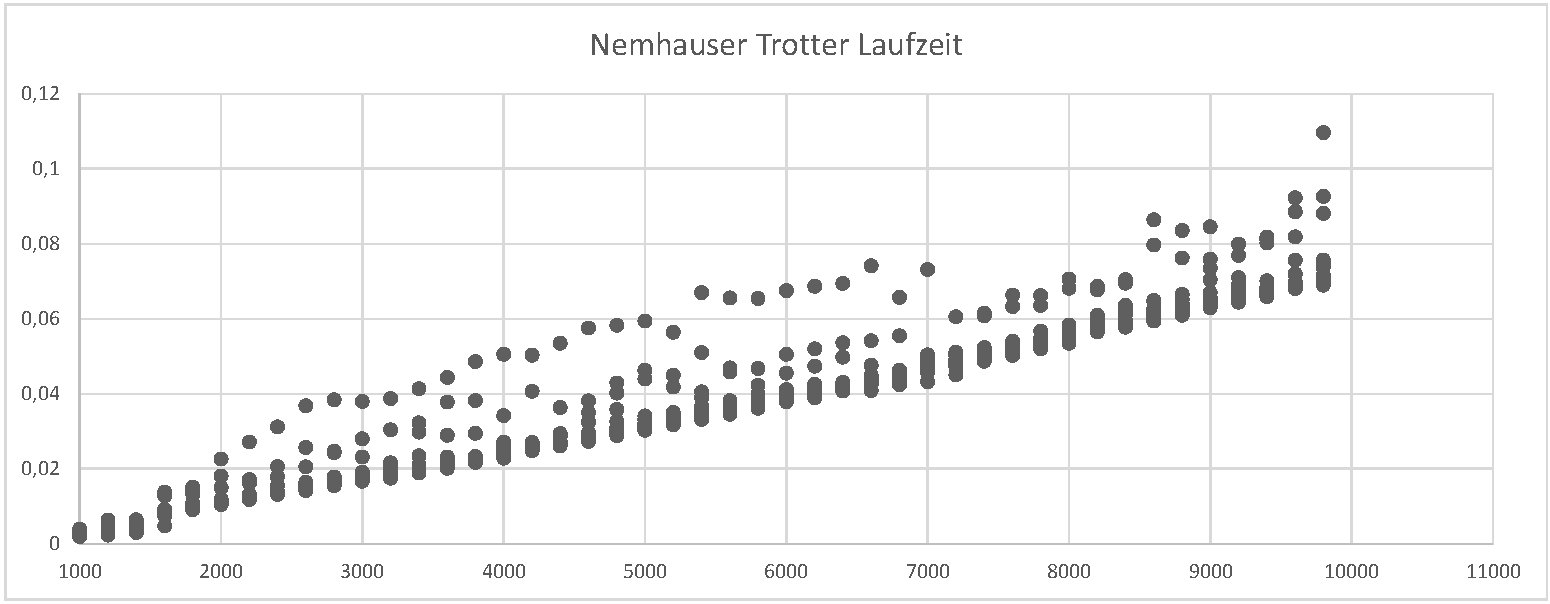
\includegraphics[width=0.7\textwidth]{trottTimeCrop.pdf}}
	\caption{Laufzeit der Nemhauser-Trotter-Regel am Testset\label{fig:trottTime}}
\centering
\end{figure}Wie in Abbildung \ref{fig:trottTime} zu sehen ist, verhält sich die Laufzeit des implementierten Algorithmus' entsprechend der Abschätzung linear zur Eingabe. Jeder Punkt repräsentiert einen Graphen, für den auf der X-Achse die entsprechende Kantenanzahl und auf der Y-Achse die Zeit, für ein Durchlauf der Nemhauser-Trotter-Regel im Schnitt für diesen Graphen in Sekunden gebraucht hat. Selbiges gilt für die Abbildung \ref{fig:crownTime}, allerdings für die Kronenregel.
%% ==============================
\section{Kronenregel}
%% ==============================
\label{ch:Grundlagen:sec:Kronenregel}
Ziel der Kronenregel ist, im Problemgraphen eine Krone zu finden, welche sich folgendermaßen definiert:\\
\textit{Für einen Graphen} $G=(V,E)$ \textit{besteht eine Krone aus} $H \subseteq V\ und\ I \subseteq V\ mit\ H \cap I = \emptyset,\ sodass$ 
\begin{enumerate}
\item $H = N(I),$ 
\item $\textit{I ein Indipendent Set ist, was bedeutet: }\forall v, w \in I\ gilt\ (vw) \notin E\ und$
\item \textit{die Kanten zwischen H und I enthalten ein Matching in dem alle Knoten aus H enthalten sind.}
\end{enumerate}
Ist eine solche Krone gefunden, kann davon die Menge $H$ in eine Knotenüberdeckung für $G$ hinzugefügt werden, um den Graphen um $H$ und $I$ zu reduzieren. Dies ist für das Knotenüberdeckungsproblem sinnvoll, da $I$ ein Independent Set ist und damit innerhalb der Menge keine Kanten existieren. Werden also nur die Nachbarknoten, beziehungsweise $H$ in die Überdeckung aufgenommen, kann man sicher sein, dass keine Kanten vernachlässigt sind. Für die Untersuchung wurde der folgende Algorithmus implementiert:
\begin{singlespace}
\begin{algorithm}[caption={Kronenregel.}, label={alg2}]
$G = (V, E), n:= |V|, m:=|E|, d:= maximaler\ Grad\ der\ Knoten\ aus\ G$
//$M_{1}$ = Maximal Matching von $G$
$M_{1} \leftarrow \emptyset$
foreach $e \in E$ do
  $M_{1} \leftarrow M_{1} \cup e$
  Entferne $e$ und $N(e)$ aus der weiteren Betrachtung
od
$O$ $\leftarrow$ nicht gepaarte Knoten in $M_{1}$
$M_{2}$ $\leftarrow$ Maximum Matching von $B = (O, N(O), \{ uv| u \in O \wedge v \in N(O)\}) $
$I$ $\leftarrow$ nicht gepaarte Knoten aus $O$ in $M_{2}$
$I'  \leftarrow \emptyset$
while $I' \neq I$ do
  $I' \leftarrow I$
  $H \leftarrow N(I)$
  $I \leftarrow I \cup \{\forall u \in O|\exists v\in H\ (uv \in M_{2})\}$
od
return $I$
\end{algorithm}
\end{singlespace}
Um das Maximal Matching $M_{1}$ zu erstellen werden im schlimmsten Fall $m \cdot d$ Schritte benötigt, da bis zu $d$ Nachbarkanten deaktiviert werden müssen. Ist $d = 1$, so wird jede Kante aus $E$ betrachtet, beziehungsweise in $M_{1}$ aufgenommen. Gilt $|M_{1}| > k$, so kann für den Graphen keine Knotenüberdeckung  $ \leq k$ gefunden werden. Das Finden der in $M_{1}$ nicht gepaarten Knoten aus $V$ kostet $n$ Schritte. $B$ kann in etwas weniger als $\frac{nd}{2}$ erstellt werden, da $n$ bis zu $2k$ kleiner ist, allerdings fällt dies für die Worst Case Abschätzung nicht sehr schwer ins Gewicht. Um das Matching $M_{2}$ in diesem bipartiten Graphen zu finden, werden wie bei der Nemhauser-Trotter-Regel  $\sqrt{n} \cdot m$ Schritte benötigt. Ist das Matching $M_{2} > k$, so kann für den Graphen keine Knotenüberdeckung  $ \leq k$ gefunden werden. Die Zeilen 8 bis 13 kosten maximal $n \cdot d$, da die Knoten aus $O$ und deren Nachbarknoten überprüft werden müssen. Insgesamt ergibt das eine Abschätzung von:
\begin{align}
&\ m \cdot d + n + \frac{nd}{2} + \sqrt{n} \cdot m + n  + n \cdot d \\
=&\ d (m+n) +2 n + \frac{nd}{2} + \sqrt{n} \cdot m \\
\Rightarrow &\ O(\sqrt{n} \cdot m)
\end{align}
Wieder erhält man $O(\sqrt{n} \cdot m)$, wird $d$ als Kontsante betrachtet, der Algorithmus eignet sich also für eine Vorverarbeitung des Graphen in Polynomialzeit. Für das Matching $M_{1}$ wird ein Maximal Matching vermutlich wegen der schnelleren Laufzeit, als das Finden eines Maximum Matchings in einem allgemeinen Graph verwendet. Allerdeings gibt es nach Blum \cite{paper:8} einen Algorithmus, der ein Maxmimum Matching in einem allgemeinen Graphen in $O(\sqrt{n} \cdot m)$ findet, was die Gesamtlaufzeit der Kronenregel zwar um den Faktor 2 verschlechtern, allerdings eventuell das Ergebnis der Reduktion verbessern würde. Abu-Khzam et al. \cite{paper:7} vermutet, dass das Matching $M_{1}$ einen großen Einfluss auf das Ergebnis der Reduktion hat, geht aber in seinem Artikel nicht weiter darauf ein. Insgesamt kann mit der Kronenregel ein Problemkern mit einer Knotenmenge von bis zu $3k$ erreicht werden.
\begin{figure}[htb]
\centering
  	{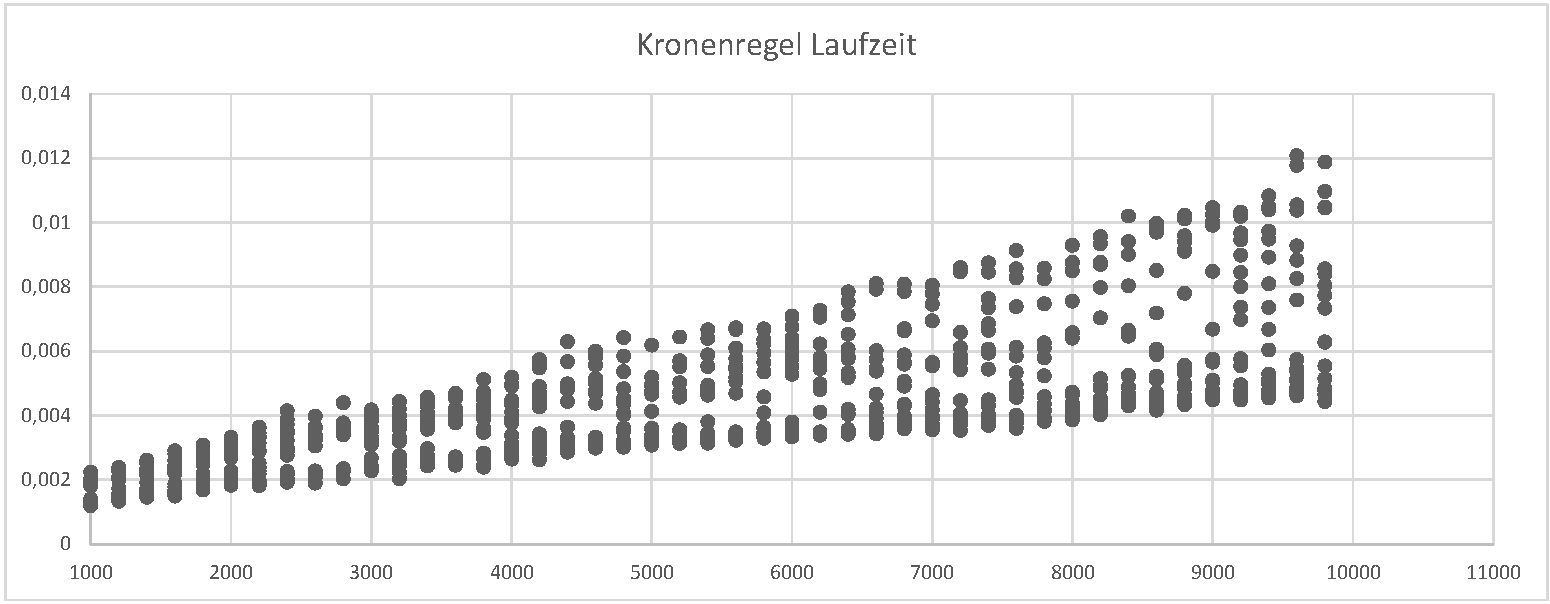
\includegraphics[width=0.7\textwidth]{crownTimeCrop.pdf}}
	\caption{Laufzeit der Kronenregel am Testset\label{fig:crownTime}}
\centering
\end{figure}
Wie in Abbildung \ref{fig:crownTime} zu sehen ist, verhält sich die Laufzeit des implementierten Algorithmus' entsprechend der Abschätzung linear zur Eingabe.
%%% Local Variables: 
%%% mode: latex
%%% TeX-master: "thesis"
%%% End: 
  % Grundlagen
%% analyse.tex
%% $Id: analyse.tex 61 2012-05-03 13:58:03Z bless $

\chapter{Analyse}
\label{ch:Analyse}
%% ==============================




%% ==============================
\section{Anforderungen}
%% ==============================
\label{ch:Analyse:sec:Anforderungen}

Um einen Graphen, der zur Diskussion steht auf einen Problemkern zu reduzieren können also wie zuvor gezeigt, verschiedene Reduktionsregeln verwendet werden. \\
Zunächst werden die Regeln anhand der folgenden Kriterien verglichen:
\begin{itemize}
	\item Laufzeit
	\item Erwartete Reduktion
	%\item Wie gut ist das Ergebnis im Vergleich zu anderen Algorithmen?	
\end{itemize}
Dann wird die Anwendung und der Effekt der Regeln auf das eigens erstellte Testset untersucht, um folgende Fragen zu beantworten:
\begin{itemize}
\item Wie effektiv sind die Reduktionsregeln in der Anwendung?
	\begin{itemize}
		\item Wie oft sind die Regeln anwendbar?
		\item Wie viel wird reduziert?
	\end{itemize}
\item Wie (gut) funktionieren die Reduktionsregeln in Kombination?
\item Wie sehen Graphen aus, auf die keine Regel anwendbar ist?
\item Wie sehen Graphen aus, auf die genau eine Regel anwendbar ist?
\end{itemize}

%% ==============================
\section{Bewertung der Reduktionsregeln}
%% ==============================
\label{ch:Analyse:sec:Berwertung}

Für jede Regel wird vorausgesetzt, dass zusätzlich zur Regel selbst alle Kanten des Grades 0 aus dem Graphen entfernt werden. Ist dies nicht der Fall, werden zum Beispiel nach der Anwendung der Buss-Regel beliebig viele Knoten mit Grad 0 übrig bleiben und die Knotenmenge der reduzierten Instanz kann nicht durch $k$ abgeschätzt werden.
In Tabelle \ref{tab:liste} stehen die Laufzeiten in der $O$-Notation und die erwartete obere Grenze der Knotenanzahl des reduzierten Problemkerns der Nemhauser-Trotter-Regel, der Kronenregel und die der Buss-Regel gegenüber. Zwar zeigte sich bei der Analyse der Laufzeit der Algorithmen, dass die Laufzeit der Nemhauser-Trotter-Regel um einige ganzzahlige Faktoren länger ist, als die der Kronenregel, allerdings hängt diese bei beiden überwiegend vom Finden von Matchings ab. 
Im folgenden Abschnitt wird betrachtet, wie sich die Reduktionsregeln in der Praxis verhalten. Zu erwarten ist, dass die Nemhauser-Trotter-Regel mehr Knoten aus den Graphen entfernt, als die Kronenregel, wobei sich in den eher dünnen Graphen des Testsets womöglich viele einfache Kronen finden lassen. 

\begin{table}[htb]
\caption{Bewertung der Reduktionsregeln\label{tab:liste}}
\vspace*{1em}
\centering
\bgroup
\def\arraystretch{1.3}%  1 is the default, change whatever you need

\begin{threeparttable}

\begin{tabular}[c]{lll}
	\hline
	\multicolumn{1}{c}{\textbf{Reduktionsregel}} & 
	\multicolumn{1}{c}{\textbf{Laufzeit}} & 
	\multicolumn{1}{c}{\textbf{Reduktion}} \\ 
	
	\hline

	Nemhauser-Trotter&$O(\sqrt{n} \cdot m)$&  $\leq 2k$\\
	Kronenregel&$O(\sqrt{n} \cdot m)$ & $\leq 3k$\\
	Buss&$O(k \cdot n)$  & $\leq k^{2}$\\
	\hline
\end{tabular}

\begin{tablenotes}\footnotesize
\item Für einen Problemgraphen $G=(V,E)$ ist \emph{k} die obere Schranke für die Größe einer Knotenüberdeckung, $n=|V|$ und $m=|E|$
\item \emph{Reduktion} bezieht sich hier auf den übrig bleibenden Problemkern nach der Reduktion
\end{tablenotes}

\end{threeparttable}

\egroup

\end{table}

%% ==============================
\section{Methodik}
%% ==============================
\label{ch:Analyse:sec:Methodik}
%% ==============================
Das Testset an dem die Algorithmen angewandt wurden besteht aus ungerichteten Graphen, die jeweils eine Knotenmenge von 1000 Knoten und eine Kantenanzahl von 1000 bis 10000 (aufsteigend in 200er Schritten) umfassen. Von jeder \emph{Graphklasse}, die sich durch die Kantenmenge auszeichnet gibt es 20 Exemplare. Dadurch entsteht ein Testset von 900 Graphen. Zum Erstellen der Graphen wurde die LEDA-Funktion \lstinline{random_simple_undirected_graph(|V|,|E|)} \cite{manual} verwendet. Da Zufallsgraphen verwendet werden, gibt es keine Vorgabe für den Parameter \emph{k}. Die obere Beschränkung der Kantenmenge (10000) hat sich bei den Tests ergeben, da ab einer bestimmten Dichte, beziehungsweise Knotenanzahl keine Reduktionsregel mehr erfolgreich ist, beziehungsweise keine Änderung am eingegebenen Graphen mehr erzielte. Dies kann mit der erwarteten Reduktion (siehe Tabelle \ref{tab:liste}) erklärt werden: Je dichter der Graph wird, desto größer wird \emph{k} und sobald $k>\frac{|V|}{2}$ wird, ist bei der Nemhauser-Trotter-Regel und somit auch bei den anderen die theoretische Größe des reduzierten Problemkerns größer oder gleich der Menge der Knoten, was bedeutet, dass theoretisch keine Reduktion stattfinden kann. Es eignen sich viele Benchmarktests \footnote{http://dimacs.rutgers.edu/pub/challenge/graph/benchmarks/} \footnote{http://sites.nlsde.buaa.edu.cn/~kexu/benchmarks/graph-benchmarks.htm} nicht, da sich diese durch sehr schwere Probleme mit dichten Graphen und Werten für \emph{k}, die sich der Größe der Knotenmenge im jeweiligen Problem annähern, auszeichnen. Eine Knotenmenge von 1000 Knoten pro Graph für das Testset erwies sich bei der Anwendung als ausreichend hoher Wert, um das Einsetzen der Reduktionsregeln zu beobachten.\\
Die Reduktionsregeln wurden jeweils solange auf einen Graphen angewandt, bis sich keine Änderungen mehr ergeben haben. Erzielte mindestens eine der Regeln eine Reduktion, wurde der gesamte Vorgang wiederholt. In der Anwendung sorgte dies dafür, dass für manche Regeln einige weitere Iterationen, beziehungsweise Durchläufe möglich wurden. In Tabelle \ref{tab:crownSpecial} ist dieser Effekt zu beobachten. Die Anwendung der Grad$_{1}$-Regel nach der Kronenregel sorgte dafür, dass bei Graph$_{1}$ 3 und bei Graph$_{2}$ sogar 5 weitere Iterationen der Kronenregel eine Reduktion erzielten.
%% ==============================
\section{Anwendung der Reduktionsregeln}
%% ==============================
\label{ch:Analyse:sec:Anwendung}
%% ==============================

Ausgeführt wurden die Experimente auf einem 2.6 GHz, Zweikern, Intel Core i5-3320M mit 8 GB Arbeitsspeicher. In der Tabelle \ref{tab:anwendung} werden die durchschnittliche Anzahl der Anwendungen pro Graph, die durchschnittliche Reduktion (Anzahl der Knoten, die aus dem Graphen entfernt wurden), und die durchschnittliche CPU-Zeit in Sekunden, die ein Durchlauf im Schnitt pro Graph gedauert hat. Die Buss-Regel wurde von der Untersuchung ausgeschlossen, da kein Wert für \emph{k} vorliegt, welcher für deren Anwendung essentiell ist, während die restlichen Regeln auch ohne diesen Parameter verwendbar sind.\\
Tabelle \ref{tab:anwendung} spiegelt die erwarteten Werte (Tabelle \ref{tab:liste}) in soweit wieder, als das die Nemhauser-Trotter-Regel eine deutlich bessere Reduktion als die Kronenregel erreicht, zumindest, wenn sie einzeln angewandt wird. Dabei werden weniger Durchläufe, allerdings ein höherer Rechenaufwand benötigt.

\begin{table}[htb]
\caption{Anwendung einzelner Reduktionsregeln\label{tab:anwendung}}
\vspace*{1em}
\centering

\bgroup
\def\arraystretch{1.3}%  1 is the default, change whatever you need

\begin{threeparttable}

\begin{tabular}[c]{llll}
	\hline
	\multicolumn{1}{c}{\textbf{Reduktionsregel}} & 
	\multicolumn{1}{c}{\textbf{Anwendungen}} & 
	\multicolumn{1}{c}{\textbf{Reduktion}} & 
	\multicolumn{1}{c}{\textbf{CPU-Zeit }} \\ 
	
	\hline

	Nemhauser-Trotter& 0.27 &  50.3 & 0.014s\\
	Kronenregel& 0.46 & 19.77 & 0.005s\\
	Grad 1&1.32 & 99.06 & 0.001s\\
	%Grad 2&$O(n|V|)\ mit\ n\leq1$&\\
	\hline
\end{tabular}

\begin{tablenotes}\footnotesize
\item Pro Zeile ist die jeweilige Reduktionsregel und den Durchschnitt pro Graph im Testset zu sehen. \emph{Anwendungen} beschreibt, wie oft nach einem Durchlauf mindestens ein Knoten entfernt wurde; \emph{Reduktion}, wie viele Knoten insgesamt pro Graph; \emph{CPU-Zeit} in Sekunden die ein Durchlauf im Schnitt pro Graph gedauert hat.
\end{tablenotes}

\end{threeparttable}

\egroup

\end{table}
Während sich die Reduktion durch die Nemhauser-Trotter und die Grad 1 Regel bei der Anwendung an dichteren Graphen, also Graphen mit einer höheren Kantenzahl, erwartungsgemäß stetig verringerte, zeigten sich bei der Kronenregel einige Ausnahmen. Wie in Abbildung \ref{fig:crown} zu sehen ist, setzten sich einige wenige Graphen deutlich vom Durchschnitt ab. In Tabelle \ref{tab:crownSpecial} werden die drei Graphen mit einer Kantenmenge über (beziehungsweise gleich) 3000 und einer durch die Kronenregel erreichten Reduktion > 480 Knoten betrachtet. Keiner dieser Graphen ist bipartit oder regulär.
Bei allen drei Graphen führte die Anwendung der Nemhauser-Trotter-Regel zu keinerlei nennenswertem Effekt, weder isoliert, noch in Kombination mit den anderen Regeln. Ähnlich verhielt sich zunächst die Grad$_{1}$-Regel, wohingegen die Anwendung in Kombination einen großen Einfluss auf die Reduktion hatte. Werden die Regeln kombiniert, scheint die Reihenfolge, in der sie eingesetzt werden schwer ins Gewicht zu fallen. Besonders fiel das bei Graph$_{1}$ (3200 Kanten) auf. Wurde zuerst die Grad$_{1}$ und dann die Kronenregel verwendet, war jeweils lediglich ein Durchlauf (Anwendung) zu beobachten. Die Grad$_{1}$-Regel scheint den Graphen derart zu verändern, dass die Struktur keine Reduktion durch die Kronenregeln mehr zulässt. Das Ergebnis von Graph$_{2}$, erzeugte die Anwendung in gerade dieser Reihenfolge eine Lösung des Problems: 1000 von 1000 Konten reduziert, wovon 619 eine Knotenüberdeckung für Graph$_{2}$ bilden. Auch hier war die Reihenfolge wieder wichtig, wie bei der Reduktionsmenge beim entgegengesetzten Experiment zu sehen ist (erst Kronenregel, dann Grad$_{1}$-Regel), wo 858 Knoten bei der Reduktion aus dem Graphen entfernt wurden. Bei Graph$_{1}$ und Graph$_{3}$ zeichnet sich der übrig gebliebene Problemkern nach der jeweils größten Reduktion dadurch aus, dass der Großteil der Knoten vom Grad 2 ist. Der Problemkern $G'_{3}$ von Graph$_{3}$, zu sehen in  Abbildung \ref{fig:crownRest}, lässt sich in die Knotenmengen $V_{1}$ und $V_{2}$  mit $|V_{1}| = |V_{2}| = 5$ aufteilen. Bis auf die Knoten $v_{1} \in V_{1}$ und $v_{2} \in V_{2}$, welche vom Grad 3 sind, hat jeder andere Knoten in  $G'_{3}$ durch die vorherige Reduktion den Grad 2. Für  $v_{1}$ und $v_{2}$ existiert eine Kante $(v_{1}, v_{2})$ in $G'_{3}$, welche die Knotenmengen verbindet. Innerhalb der Knotenmengen existiert einen Zyklus (Kreis), mit ungerader Knotenzahl, woraus sich folgern lässt, dass $G'_{3}$ nicht bipartit ist. Hier ist keine der Reduktionsregeln mehr erfolgreich.
\begin{figure}[htb]
\centering
  	{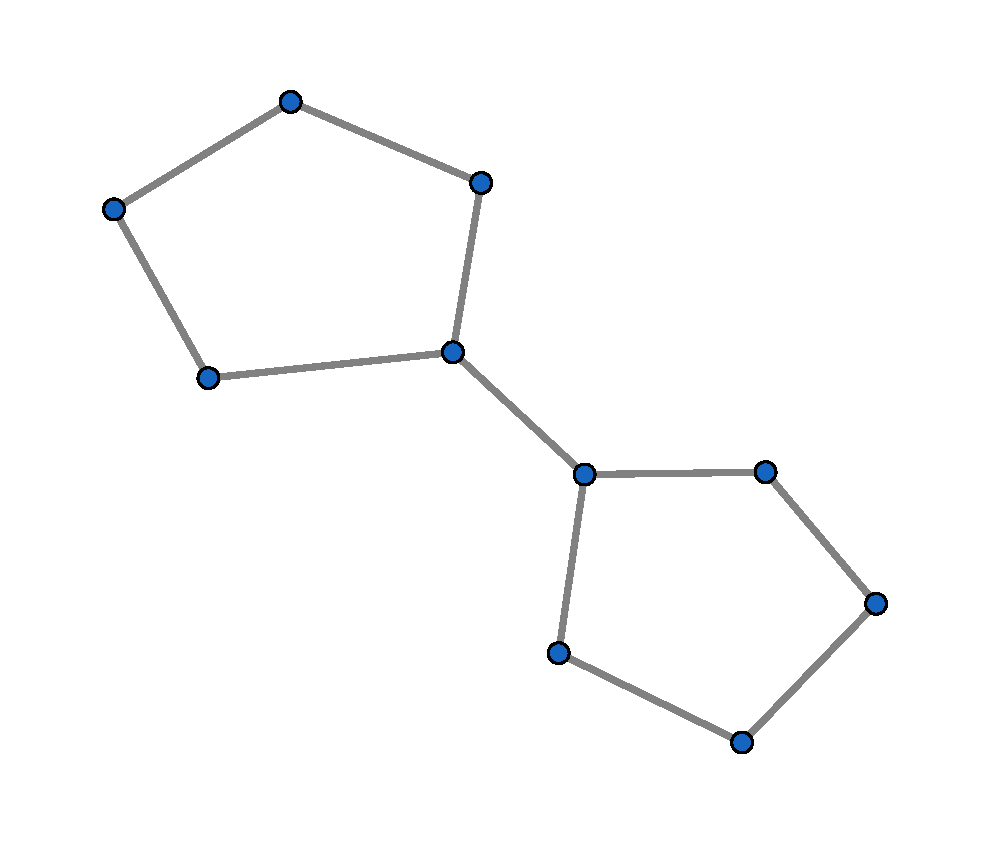
\includegraphics[width=0.3\textwidth]{crownRest.pdf}}
	\caption{Graph$_{3}$ nach Anwendung von Grad$_{1}$-Regel und Kronenregel.\label{fig:crownRest}}
\centering
\end{figure}

\begin{figure}[htb]
\centering
  	{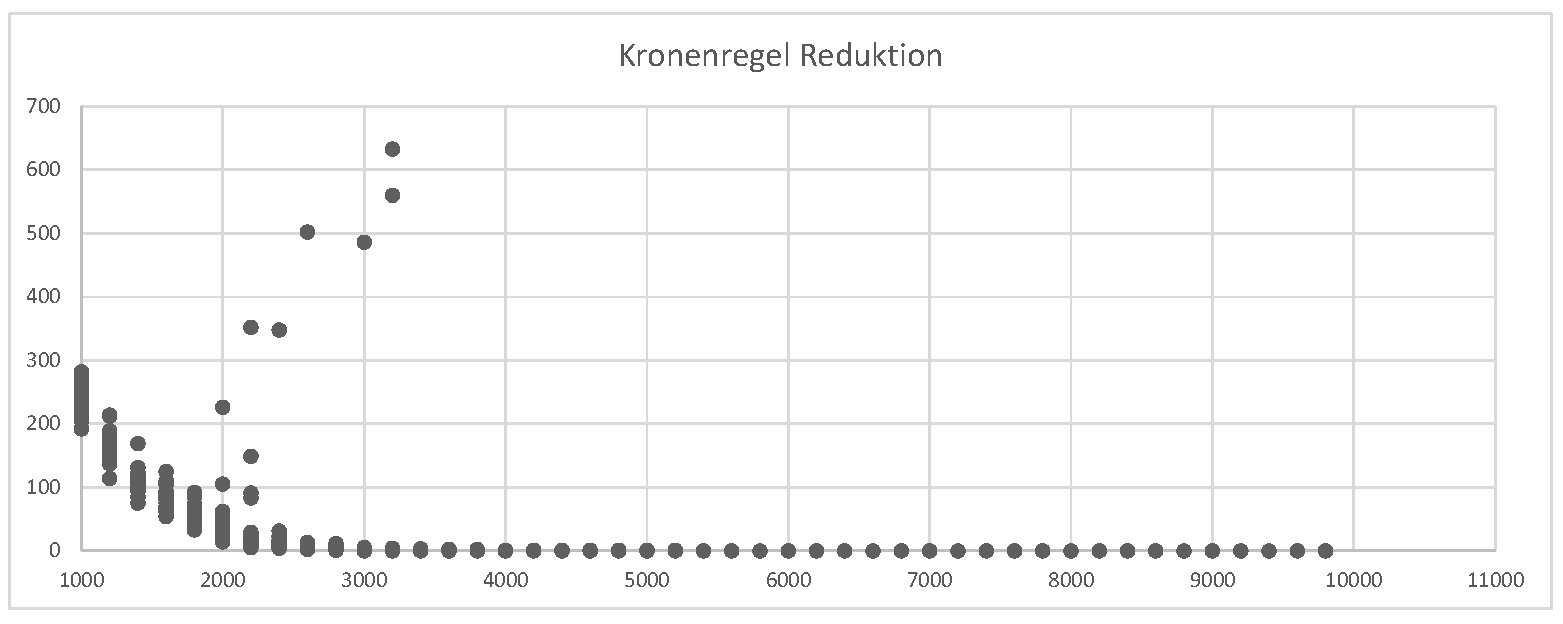
\includegraphics[width=\textwidth]{analysisCrown.pdf}}
	\caption{Anwendung der Kronenregel.\label{fig:crown}}
\centering
\end{figure}

\begin{table}[htb]
\caption{Besondere Graphen für die Kronenregel \label{tab:crownSpecial}}
\vspace*{1em}
\centering

\bgroup
\def\arraystretch{1.3}%  1 is the default, change whatever you need

\begin{threeparttable}

\begin{tabular}[c]{lllll}
	\hline
	\multicolumn{1}{c}{\textbf{Graph}} & 
	\multicolumn{1}{c}{\textbf{Reduktionsregeln}} & 
	\multicolumn{1}{c}{\textbf{Anwendungen$_{1}$}} &
	\multicolumn{1}{c}{\textbf{Anwendungen$_{2}$}} &
	\multicolumn{1}{c}{\textbf{Reduktion}} \\ 
	
	\hline
		
	Graph$_{1}$ & Kronenregel& 11 & - & 560\\
	& Nemhauser-Trotter & 1 & - & 4\\
	& Grad$_{1}$ & 1 & - & 18 \\
	& Grad$_{1}$-Kronenregel & 1 & 1 & 22\\
	& Kronenregel - Grad$_{1}$ & 14 & 11 & 946\\
	
	\hline

	Graph$_{2}$ & Kronenregel & 13 & - & 486\\
	& Nemhauser-Trotter & 1 & - & 6\\
	& Grad$_{1}$ & 2 & - & 40 \\
	& Grad$_{1}$-Kronenregel & 12 & 13 & 1000\\
	& Kronenregel - Grad$_{1}$ & 18 & 12 & 858\\

	\hline	
	
	Graph$_{3}$ & Kronenregel & 15 & - &633\\	
	& Nemhauser-Trotter & 1 & - & 4\\
	& Grad$_{1}$ & 2 & - & 46 \\
	& Grad$_{1}$-Kronenregel & 18 & 11 & 990\\
	& Kronenregel - Grad$_{1}$ & 15 & 9 & 971\\
	
	\hline

	
	
\end{tabular}
\begin{tablenotes}\footnotesize
\item  Durchschnittliche Anzahl der Anwendungen der Regeln und der Durchschnitt der entfernten Knoten pro Graph für die verschiedenen Kombinationen von Regeln für die besonderen Graphen der Kronenregel-Reduktion
\end{tablenotes}

\end{threeparttable}

\egroup

\end{table}

Die in Tabelle \ref{tab:kombination} zusammengefassten Ergebnisse zeigen, dass die Nemhauser-Trotter-Regel in Kombination mit anderen Regeln nicht die gleiche Reduktion erzeugt, wie Grad$_{1}$ und Kronenregel. Des Weiteren lassen sich eine Reihe von Beobachtungen anstellen.
\begin{figure}[htb]
\centering
  	{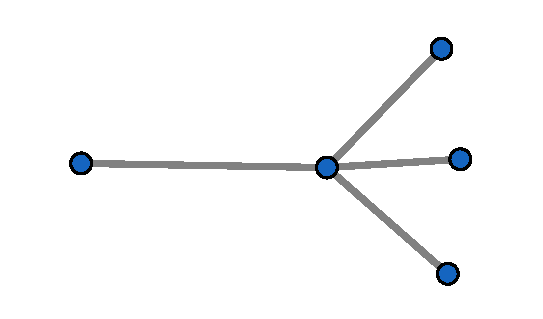
\includegraphics[width=0.3\textwidth]{restkrone.pdf}}
	\caption{Einfache Krone\label{fig:restcrown}}
\centering
\end{figure}
\\
Da durch die Grad$_{1}$-Regel einfache 1-gradige Knoten, beziehungsweise deren Nachbarn und damit der Kopf einer einfachen Krone, reduziert wird, stellt sie eine vereinfachte Form der Kronenregel dar. Daher sollten intuitiv nach der erschöpfenden Anwendung der Kronenregel kaum Probleminstanzen, bei denen die Grad$_{1}$-Regel erfolgreich ist, übrig bleiben. Wie die Tabelle allerdings zeigt, ist die Kombination beider Regeln im Vergleich zu den anderen Zweierkombination diejenige, die im Durchschnitt am meisten Knoten aus den Problemgraphen entfernt. Zu dem besseren Ergebnis der Reduktion kommt hier noch die stark erhöhte durchschnittliche Anwendung pro Graph. Ein Grund hierfür könnte die Auswahl des ersten Matchings in der Kronenregel sein, welches maßgeblich für die darauffolgende Reduktion ist. Eine einfache Krone, wie sie in Abbildung \ref{fig:crownRest} zu sehen ist, wird mit großer Wahrscheinlichkeit von der Kronenregel, so wie sie hier verwendet wird, ignoriert. Im Abschnitt \ref{ch:Implementierung:sec:Kronenregel} wird genauer erläutert, warum das der Fall ist: Bei der Anwendung auf das Testset wird die größte Reduktion mit der Kronenregel dann erreicht, wenn bei der Erstellung des Matchings $M_{1}$ zunächst Kanten betrachtet werden, bei denen beide Knoten höhergradig, genauer gesagt einen höheren Grad, als der durchschnittliche Knoten im aktuellen Graphen haben. Wäre die abgebildete Krone Teil eines größeren Graphen, kann es sein, dass der Kopf dieser Krone nicht in das Matching $M_{1}$ aufgenommen und so bei der weiteren Reduktion nicht berücksichtigt wird. Die Grad$_{1}$-Regel reduziert demnach jene einfachen Kronen, die von der Kronenregel ignoriert, beziehungsweise nicht erkannt werden. Wird nun die Reihenfolge geändert, in der die beiden Regeln angewandt werden, zeigen sich nur minimale Änderungen in der durchschnittlichen Reduktion und der durchschnittlichen Anwendung pro Graph. Entgegen der Beobachtung für die Sonderfälle bei der Anwendung der Kronenregel zeigt sich im Allgemeinen, dass die Grad$_{1}$-Regel und die Kronenregel überwiegend verschiedene Arten von Kronen abdecken, da annähernd gleiche Ergebnisse unabhängig von der Reihenfolge der Regeln erzielt werden. Die Unterschiede in den Ergebnissen zeichnen sich dadurch aus, dass die als Zweites verwendete Regel im Schnitt weniger Anwendungen hat, als wenn sie Erstes verwendet wird. Für die Kronenregel bedeutet das im Schnitt eine Differenz von 0.42 Durchläufen pro Graph, für die Grad$_{1}$-Regel nur 0.07. Diese 0.07 Durchläufe der Grad$_{1}$-Regel mehr pro Graph verschlechtern allerdings die Gesamtreduktion. Diesen Effekt kann auch bei dem Extrembeispiel von Graph${_1}$ in Tabelle \ref{tab:crownSpecial} beobachten, wo der gleiche Effekt eintritt. Es scheint also im Großteil der Fälle für eine maximale Reduktion von Vorteil zu sein, wenn die Kronenregel vor der Grad$_{1}$-Regel angewandt wird, was die anderen Beispielen in Tabelle \ref{tab:kombination} wiederum untermalen.\\ \\
Bei der Grad$_{1}$-Regel in Kombination mit der Nemhauser-Trotter-Regel sorgt die Reihenfolge zwar für einen Unterschied in der durchschnittlichen Anwendung, allerdings ist das Ergebnis der Reduktion identisch. Ein Teil der von der Grad$_{1}$-Regel abgedeckten Reduktion wird also vermutlich auch von der Nemhauser-Trotter-Regel entfernt und dem entsprechend auch anders herum. Die Differenz bei verschiedener Reihenfolge beträgt bei der Grad$_{1}$-Regel 0.2 und bei der NT-Regel 0.26 Iterationen pro Graph, was vermuten lässt, dass die Grad$_{1}$-Regel Bereiche des Graphen, wo beide Regeln greifen effizienter, mit weniger Durchläufen entfernt. Beim Vergleich von diese Kombination mit einer Grad$_{1}$-Kronenregel-Reduktion, fällt auch auf, dass die Form des Graphen, die die Nemhauser-Trotter-Regel durch das Entfernen von Knoten und Kanten erzeugt, die Anwendungsmöglichkeit der Grad$_{1}$-Regel einschränkt. In die andere Richtung scheint diese Einschränkung auch zu gelten. Die gesamte Reduktion pro Graph erhöht sich nicht sonderlich, im Vergleich zu den Werten, die die Grad$_{1}$-Regel alleine erzeugt (Tabelle \ref{tab:anwendung}). \\ \\
Kronenregel und Nemhauser-Trotter-Regel sorgen in Kombination dafür, dass die jeweilige Anwendung pro Graph leicht erhöht wird. Auch zeigt sich ein deutlicher Anstieg der Reduktion pro Graph im Vergleich zur Einzelanwendung, was darauf hindeutet, dass die beiden Regeln wiederum verschiedene Bereiche des Graphen entfernen. Bei den Dreierkombinationen zeigt sich dieser Trend ebenfalls: Wird hier die Kronenregel unmittelbar vor der Nemhauser-Trotter-Regel angewandt, finden deutlich mehr Iterationen (der NT-Regel) pro Graph statt, als es bei vorheriger Verwendung der Grad$_{1}$-Regel der Fall ist. Zwei Interessante Ergebnisse liefern die Kombinationen Grad$_{1}$ - Nemhauser-Trotter - Kronenregel und Grad$_{1}$ - Kronenregel - Nemhauser-Trotter. Die Position, beziehungsweise die Reihenfolge der Regeln beeinflusst die Anwendungshäufigkeit von Grad$_{1}$ und Nemhauser-Trotter-Regel deutlich, während Gesamtreduktion und Anwendungen der Kronenregel annähernd gleich bleiben. Dies könnte wiederum ein Indikator dafür sein, dass Nemhauser-Trotter und Grad$_{1}$-Regel ähnliche Teile des Graphen reduzieren und die Kronenregel den Graphen scheinbar für die jeweilige Reduktion günstig verändert.
Werden Nemhauser-Trotter-Regel, Kronenregel und Grad$_{1}$-Regel in dieser Reihenfolge angewandt, kann im Schnitt die größte Reduktion pro Graph erreicht werden. In Abbildung \ref{fig:trottCrownOne} lassen sich wiederum einige Ausnahmen erkennen: Zwei Graphen stechen besonders aus dem Durchschnitt heraus, zu sehen in Tabelle \ref{tab:trottCrownOneSpecial}. Zum einen ein Graph mit 2000 Kanten und einer Reduktion von lediglich 195 Knoten (Graph$_{4}$), während andere Graphen dieser Größe annähernd komplett gelöst wurden. Zum anderen ein Graph mit 7200 Kanten, bei dem 762 Knoten entfernt werden konnten (Graph$_{5}$). Keiner der Graphen ist - weder vor noch nach der Reduktion - regulär oder bipartit. Die Kronenregel greift bei Graph$_{5}$ nur, wenn die Grad$_{1}$-Regel den einen eingradigen und dessen Nachbarknoten entfernt. Bis auf die Grad$_{1}$-Regel kann keine Reduktionsregel auch nur einen Knoten des Graphen entfernen, wenn sie alleine angewandt werden. Eine weitere interessante Beobachtung für Graph$_{5}$ ist, dass die Konfiguration für die Kronenregel sehr wichtig für eine hohe Reduktion ist. Die Knoten des Graphen haben vor der Reduktion einen durchschnittlichen Grad von 14 (abgerundet). Werden beim finden des Matchings $M_{1}$ zunächst Kanten, bei denen jeder Knoten den Grad $\geq$ 14 hat bevorzugt, findet keine Reduktion statt, auch nicht in Kombination mit den anderen Regeln. Wird als Einschränkung stattdessen einen Grad > 14 gewählt, werden 702 Knoten reduziert. Das Beste Ergebnis wird bei einer Konfiguration erreicht, bei der der Grad beider Knoten größer, als der durchschnittliche Grad aller Knoten ist. Auf dieses Phänomen wird in Kapitel \ref{ch:Implementierung:sec:Kronenregel} weiter eingegangen. Bei Graph$_{4}$ zeigt sich, wie bei Graph$_{5}$, dass die Nemhauser-Trotter-Regel keinen Einfluss auf die Gesamtreduktion hat. Kronenregel und Grad$_{1}$-Regel entfernen in Kombination die Größte Menge an Knoten.


\begin{figure}[htb]
\centering
  	{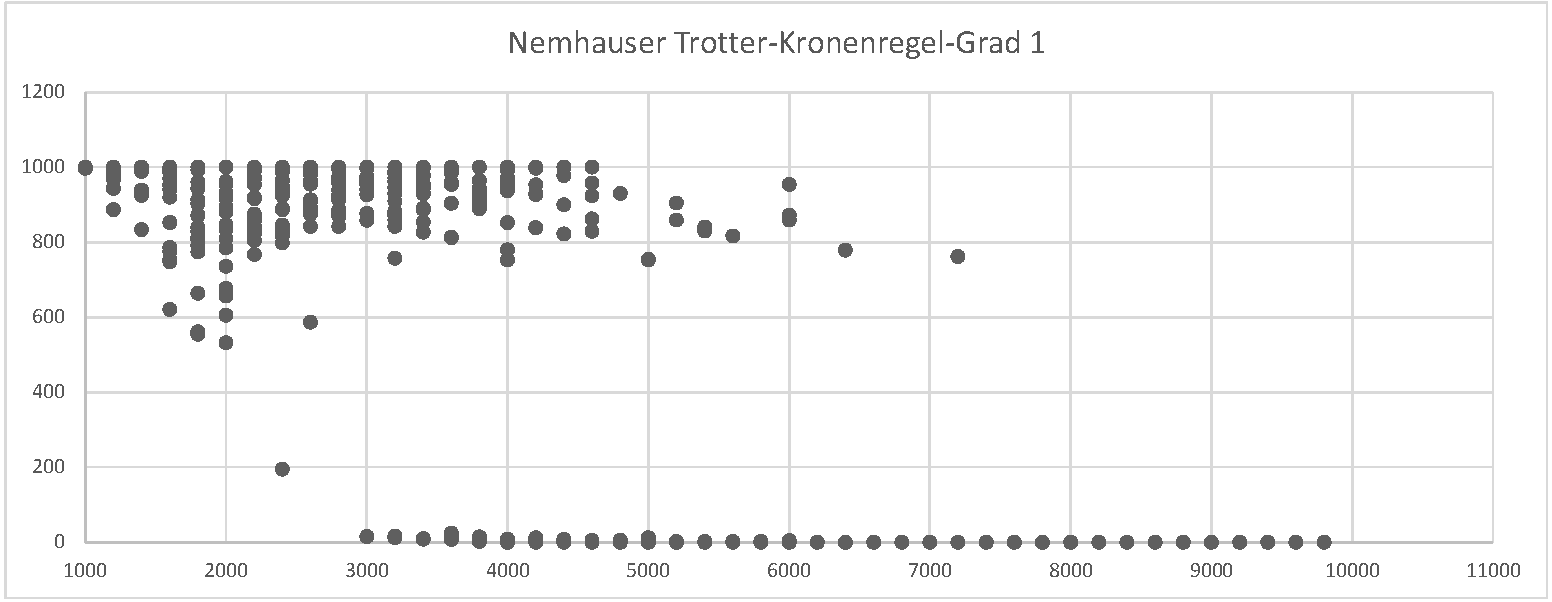
\includegraphics[width=\textwidth]{analysisTrott_Crown_One.pdf}}
	\caption{Anwendung von Nemhauser-Trotter-Regel, Kronenregel und Grad$_{1}$-Regel.\label{fig:trottCrownOne}}
\centering
\end{figure}


\begin{table}[htbp]
\caption{Anwendung kombinierter Reduktionsregeln\label{tab:kombination}}
\vspace*{1em}
\centering

\bgroup
\def\arraystretch{1.3}%  1 is the default, change whatever you need

\begin{threeparttable}

\begin{tabular}[c]{l l l l l}
	\hline
	\multicolumn{1}{c}{\textbf{Kombination}} &
	\multicolumn{1}{c}{\textbf{Anwendungen$_{1}$}} &
	\multicolumn{1}{c}{\textbf{Anwendungen$_{2}$}} &
	\multicolumn{1}{c}{\textbf{Anwendungen$_{3}$}} & 
	\multicolumn{1}{c}{\textbf{Reduktion}} \\
	\hline

	K - G$_{1}$ & 3.63 & 4.3 & - &331.8\\
	G$_{1}$ - K & 4.37 & 3.22 & - &331.17\\
	K - NT & 0.8 & 0.38 & - & 68.28 \\
	NT - K & 0.45 & 0.56 & - & 68.6\\
	G$_{1}$ - NT & 1.33 & 0.017 & - & 99.87\\
	NT - G$_{1}$ & 0.28 & 1.13 & - & 99.87\\
	K  - G$_{1}$ - NT & 3.61 & 4.29 & 0.11 & 334.67 \\
	K - NT - G$_{1}$ & 3.6 & 0.87 & 3.39 & 334.83 \\
	G$_{1}$ - NT - K & 4.36 & 0.12 & 3.2 & 334.17 \\
	G$_{1}$ - K - NT & 3.61 & 3.2 & 0.65 & 334.16 \\
	NT - K - G$_{1}$ & 0.39 & 3.44 & 4.03 & 335.2 \\
	NT - G$_{1}$ - K & 0.91 & 3.42 & 3.2 & 334.16 \\
	\hline
	
\end{tabular}

\begin{tablenotes}\footnotesize
\item  Durchschnittliche Anzahl der Anwendungen der Regeln und der Durchschnitt der entfernten Knoten pro Graph für die verschiedenen Kombinationen von Regeln
\end{tablenotes}

\end{threeparttable}

\egroup

\end{table}


\begin{table}[htb]
\caption{Besondere Graphen für die Dreierkombinationen von Regeln\label{tab:trottCrownOneSpecial}}
\vspace*{1em}
\centering

\bgroup
\def\arraystretch{1.3}%  1 is the default, change whatever you need

\begin{threeparttable}

\begin{tabular}[c]{llllll}
	
	\hline
	\multicolumn{1}{c}{\textbf{Graph}} & 
	\multicolumn{1}{c}{\textbf{Reduktionsregeln}} & 
	\multicolumn{1}{c}{\textbf{Anwend.$_{1}$}} &
	\multicolumn{1}{c}{\textbf{Anwend.$_{2}$}} &
	\multicolumn{1}{c}{\textbf{Anwend.$_{3}$}} &
	\multicolumn{1}{c}{\textbf{Reduktion}} \\ 
	
	\hline
		
	Graph$_{4}$ & NT - K - G$_{1}$ & 1 & 5 & 6 & 195 \\
	& G$_{1}$ - NT - K & 6 & 0 & 5 & 195 \\
	& Nemhauser-Trotter & 1 & - & - & 11 \\
	& Kronenregel & 1 & - & - & 11 \\
	& Grad$_{1}$ & 2 & - & - & 91 \\
	& Kronenregel - Grad$_{1}$ & 6 & 5 & - & 195 \\
	
	\hline

	Graph$_{5}$ & NT - K - G$_{1}$ & 1 & 9 & 2 & 762 \\
	& Nemhauser-Trotter & 0 & - & - & 0\\
	& Kronenregel & 0 & - & - & 0\\
	& Grad$_{1}$ & 1 & - & - & 2 \\
	& Kronenregel - Grad$_{1}$ & 9 & 3 & - & 762\\
	\hline
	
\end{tabular}
\begin{tablenotes}\footnotesize
\item  Anzahl der Anwendungen der Kombinationen der Regeln und die Summe der entfernten Knoten für die besonderen Graphen der Nemhauser-Trotter - Kronenregel - Grad$_{1}$ - Reduktion
\end{tablenotes}

\end{threeparttable}

\egroup

\end{table}

\section{Zusammenfassung}
%% ==============================
\label{ch:Analyse:sec:Zusammenfassung}

Es hat sich gezeigt, dass die Regeln in der Einzelanwendung bei der Größe der Reduktion im Vergleich zueinander den Erwartungen aus Tabelle \ref{tab:liste} entsprechen. Allerdings wurde festgestellt, dass die Anwendbarkeit der Regeln nicht ausschließlich von der Dichte eines Graphen abhängt, sondern stark von dessen Struktur, wie am Beispiel von Graph$_{5}$ zu sehen ist, wo genau 2 Knoten entfernt werden mussten, um die Anwendung der Kronenregel zu ermöglichen. Wie erwartet, nimmt die Anzahl der reduzierten Knoten pro Graph mit wachsender dichte ab. Im schlimmsten Fall, zum Beispiel bei einer Clique, also einem (Teil-)Graphen, bei dem jeder Knoten eine Kante zu jedem anderen Knoten der Clique hat, ist keine Reduktion mehr möglich, da sich dann auch die Größe der kleinsten Knotenüberdeckung für diesen Graphen der Knotenmenge annähert.

%%% Local Variables: 
%%% mode: latex
%%% TeX-master: "thesis"
%%% End: 
     % Analyse
%% entwurf.tex
%% $Id: entwurf.tex 61 2012-05-03 13:58:03Z bless $
%%

\chapter{Entwurf / Konzeption}
\label{ch:Entwurf}
%% ==============================
In diesem Kapitel erfolgt die ausführliche Beschreibung des eigenen
Lösungsansatzes. Dabei sollten Lösungsalternativen diskutiert und
Entwurfsentscheidungen dargelegt werden.

%% ==============================
\section{Abschnitt 1}
%% ==============================
\label{ch:Entwurf:sec:Abschnitt1}

%% ==============================
\section{Abschnitt 2}
%% ==============================
\label{ch:Entwurf:sec:Abschnitt2}

%% ==============================
\section{Zusammenfassung}
%% ==============================
\label{ch:Entwurf:sec:zusammenfassung}

Am Ende sollten ggf. die wichtigsten Ergebnisse nochmal in \emph{einem}
kurzen Absatz zusammengefasst werden.

%%% Local Variables: 
%%% mode: latex
%%% TeX-master: "thesis"
%%% End: 
     % Entwurf
%% implemen.tex
%% $Id: implemen.tex 61 2012-05-03 13:58:03Z bless $
%%

\chapter{Implementierung}
\label{ch:Implementierung}
%% ==============================


Die Regeln wurden in der Programmiersprache \emph{C++} unter Verwendung der Bibliothek \emph{LEDA} \cite{manual} implementiert. Sie wurden bei der Anwendung jeweils solange wiederholt, bis sich am Graphen keine Änderung mehr ergab. 

%% ==============================
\section{Kronenregel}
%% ==============================
\label{ch:Implementierung:sec:Kronenregel}

Beim Austesten der Kronenregel hat sich gezeigt, dass die Auswahl des Matchings $M_{1}$ im in Kapitel \ref{ch:Grundlagen:sec:Kronenregel} dargestellten Algorithmus das Ergebnis der Reduktion in großem Maße beeinflusst, was bereits zuvor aufgefallen ist \cite{paper:7}. Dies ist bei der Implementierung für diese Arbeit dadurch aufgefallen, dass beim Anwenden an einem für die Kronenregel gut geeigneten Testgraphen zunächst keine Reduktion stattgefunden hat. Dieser ist in Abbildung \ref{fig:crown1} zu sehen. Um zu funktionieren, müssen die Kanten $(A,C), (D,E), (J,K), (L,B)$ für das Matching $M_{1}$ ausgewählt werden, da ansonsten zum Beispiel $K$ und $L$ nicht korrekt als Kopf der Krone, beziehungsweise nicht als der Menge $H$ zugehörig identifiziert werden.
\begin{figure}[htb]
\centering
  	{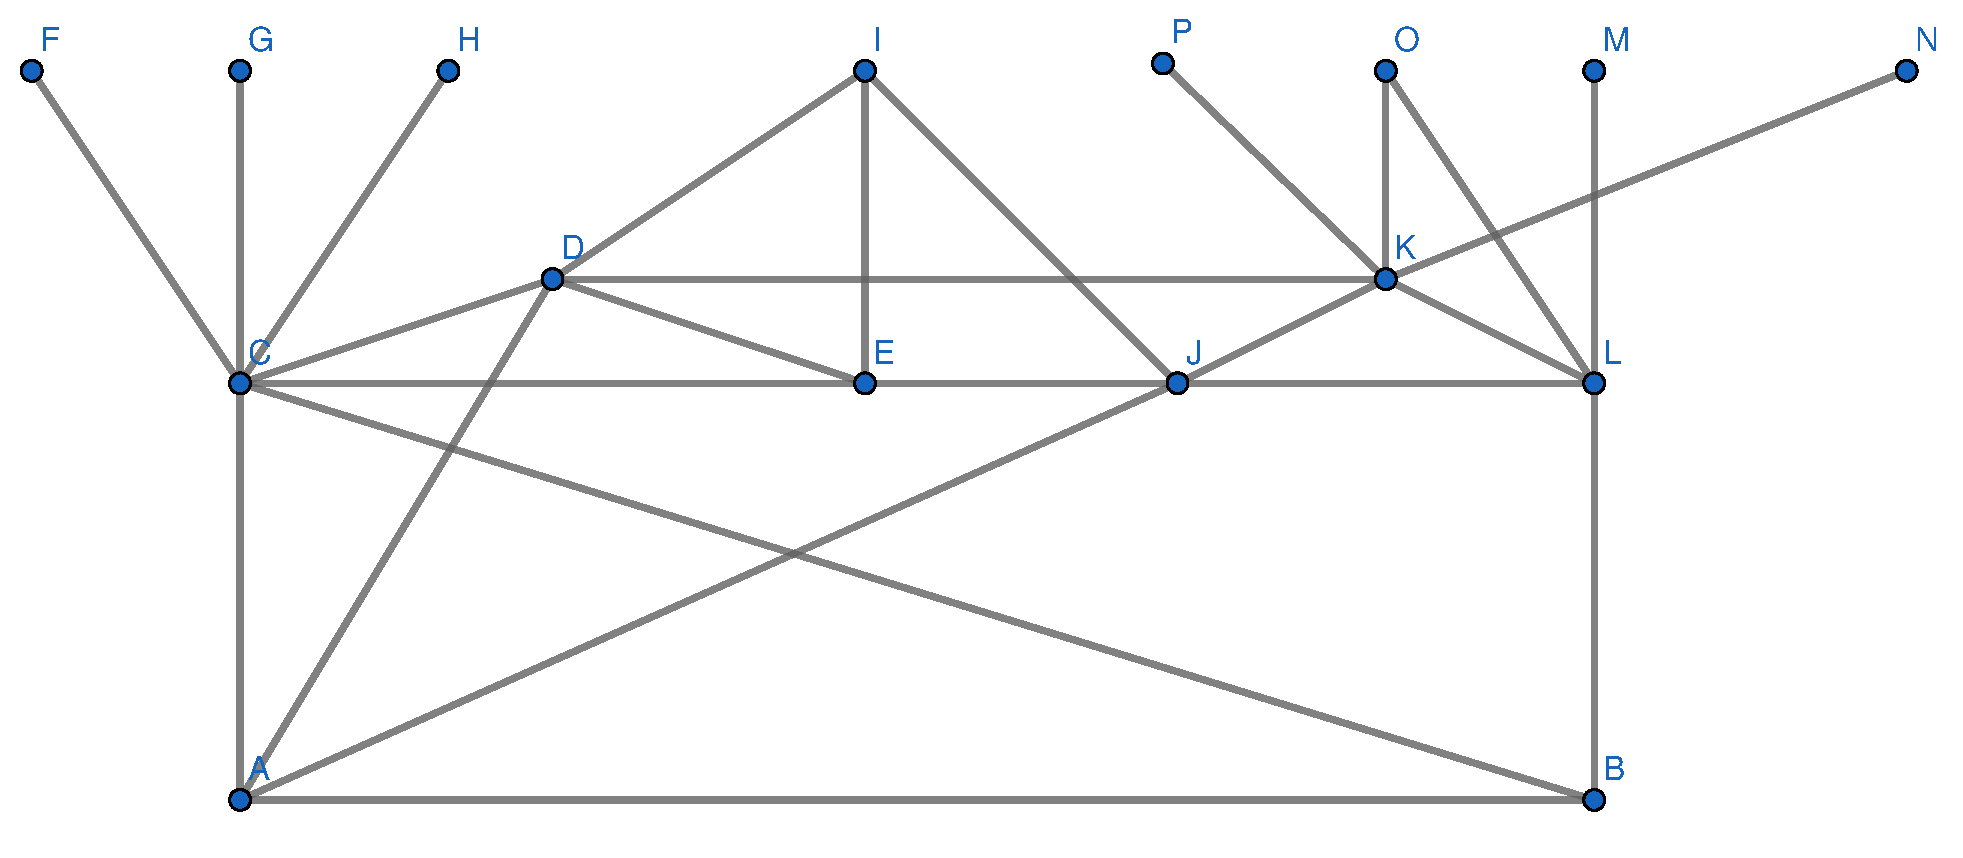
\includegraphics[width=.9\textwidth]{crown1Crop.pdf}}
	\caption{Beispielgraph für die Anwendung der Kronenregel\label{fig:crown1}}
\centering
\end{figure}
\begin{table}[htb]
\caption{Mindestens ein Knoten mit Einschränkung\label{tab:degreeOR}}
\vspace*{1em}
\centering

\bgroup
\def\arraystretch{1.3}%  1 is the default, change whatever you need

\begin{threeparttable}

\begin{tabular}[c]{lll}
	\hline
	\multicolumn{1}{c}{\textbf{Grad der Knoten}} & 
	\multicolumn{1}{c}{\textbf{Anwendungen}} & 
	\multicolumn{1}{c}{\textbf{Reduktion}} \\ 
	
	\hline

	keine Einschränkung&0.29&13.04\\
	>1&0.29 &13.04 \\
	>2&0.29 &13.22 \\
	>3& 0.27& 12.92 \\
	>4& 0.3& 13.71 \\
	>5& 0.31&13.38 \\
	>Größte Anzahl& 0.32&13.44 \\
	>Durchschnittliche Anzahl& 0.29&12.98 \\
	\hline
\end{tabular}
\begin{tablenotes}\footnotesize
\item \emph{Grad der Knoten} bezieht sich auf die Bedingung für die bevorzugte Auswahl der Kanten für $M_{1}$, bzw. dessen Knoten. \emph{Anwendung} und \emph{Reduktion} stellen jeweils den Durchschnittswert beim gesamten Testset dar.
\end{tablenotes}

\end{threeparttable}

\egroup

\end{table}

\begin{table}[htb]
\caption{Beide Knoten mit Einschränkung\label{tab:degreeAND}}
\vspace*{1em}
\centering

\bgroup
\def\arraystretch{1.3}%  1 is the default, change whatever you need

\begin{threeparttable}

\begin{tabular}[c]{lll}
	\hline
	\multicolumn{1}{c}{\textbf{Grad der Knoten}} & 
	\multicolumn{1}{c}{\textbf{Anwendungen}} & 
	\multicolumn{1}{c}{\textbf{Reduktion}} \\ 
	
	\hline

	keine Einschränkung&0.29&13.04\\
	>1&0.36 &15.34 \\
	>2&0.41 &16.96 \\
	>3& 0.39& 16.52 \\
	>4& 0.4 &15.78 \\
	>5& 0.4 & 15.72\\
	>Größte Anzahl& 0.29 &13.06 \\
	>Durchschnittliche Anzahl& 0.46&19.77 \\
	\hline
\end{tabular}
\begin{tablenotes}\footnotesize
\item \emph{Grad der Knoten} bezieht sich auf die Bedingung für die bevorzugte Auswahl der Kanten für $M_{1}$, bzw. dessen Knoten. \emph{Anwendung} und \emph{Reduktion} stellen jeweils den Durchschnittswert beim gesamten Testset dar.
\end{tablenotes}

\end{threeparttable}

\egroup

\end{table}
Wenn nun beim Finden von $M_{1}$ zunächst bevorzugt Kanten mit Knoten höheren Grades vor den anderen betrachtet werden, können bessere Ergebnisse in der darauf folgenden Reduktion erzielt werden und die richtigen Kanten werden getroffen. Daraufhin wurde untersucht, wie die höhergradigen Knoten, beziehungsweise die dazugehörigen Kanten ausgewählt werden müssen. Auf der einen Seite (Tabelle \ref{tab:degreeOR}) wurden Kanten betrachtet, bei denen das Auswahlkriterium auf mindestens einen der Knoten zutrifft, auf der anderen Seite Kanten, bei denen beide Knoten die Bedingung erfüllen (Tabelle \ref{tab:degreeAND}). Die Einschränkungen \emph{Größte Anzahl} und \emph{Durchschnittliche Anzahl} ergeben sich jeweils aus der Menge an Knoten eines bestimmtes Grades. Bei Ersterem werden Knoten, deren Grad größer ist, als der, der im aktuellen Graphen am häufigsten vorkommt bevorzugt. Bei Letzterem dementsprechend Knoten mit einem deren Grad, größer als, der der im aktuellen Graphen dem Durchschnitt entspricht. Diese Werte werden bei jeder Iteration des Algorithmus neu berechnet und passen sich dadurch während der Laufzeit an den Graphen an.\\ 
Generell wird eine bessere (größere) Reduktion mit der Kronenregel erreicht, wenn beim Matching $M_{1}$ zunächst Kanten betrachtet werden, bei denen die Einschränkung auf beide Knoten zutrifft. Die Reduktionsmenge bei Knoten mit $Grad>2$ erzeugt im Vergleich mit anderen statischen Werten das beste Ergebnis. Dies könnte damit zusammenhängen, dass bei den Graphen, bei denen diese Regel sehr effektiv ist, der durchschnittliche Grad der Knoten 2 ist und es sich damit um einen eher dünnen Graphen handelt. Vermutlich erzielt die Bevorzugung des durchschnittlichen Grades das beste Ergebnis, da sich dieser Wert mit jedem Durchlauf verändert.
Das Problem bei diesem Vorgehen ist, dass einfache Kronen ignoriert werden können, weshalb die Kombination mit der Grad$_{1}$-Regel vermutlich so gute Ergebnisse erzielt, wie in Kapitel \ref{ch:Analyse:sec:Anwendung} zu sehen ist.





%% ==============================
\section{Nemhauser-Trotter-Regel}
%% ==============================
\label{ch:Implementierung:sec:Trott}

Bei der Umsetzung des Algorithmus' der Nemhauser-Trotter-Regel sind keine Besonderheiten aufgefallen, wie es bei der Kronenregel der Fall war. Für das Erstellen des bipartiten Graphen $B$ wurden zwei Referenzarrays angelegt, sodass für jeden Knoten aus $G$ das entsprechende Paar in $B$ gefunden werden konnte und anders herum, also für jeden Knoten aus $B$ das entsprechende Urbild aufgerufen werden konnte. Die weiteren Berechnungen konnten dann mithilfe der LEDA-Funktion MAX\_CARD\_BIPARTITE\_MATCHING aus mcb\_matching.h und LEDA-Iteratoren angestellt werden. Um zu überprüfen, ob der erstelle Graph $B$ tatsächlich bipartit ist und bei der Erstellung kein Fehler unterlaufen ist, wurde eigens eine entsprechende Funktion geschrieben, da LEDA eine solche nicht bereitstellt. In dieser Funktion wird versucht, die Knoten des Graphen in zwei Farben einzufärben, sodass keine zwei benachbarten Knoten die gleiche Farbe haben. Der Algorithmus funktioniert, wie folgt:
\begin{singlespace}
\begin{algorithm}[caption={Bipartit-Check}, label={alg4}]
Eingabe: Graph $G=(V,E)$ 
foreach $ v \in V$ do
  if Farbe[$v$]=leer then do
    Farbe[$v$] $\leftarrow$ Farbe$_{1}$    
    Queue.push($v$)
    while Queue.isNotEmpty do
      $v$ $\leftarrow$ Queue.pop
      if Farbe[$N(v)$]=leer oder Farbe[$N(v)$]=$\neg$Farbe[$v$] then do
        Farbe[$N(v)$] $\leftarrow$ $\neg$Farbe[$v$]
        Queue.push($N(v)$)
      else do
        return $G$ is nicht bipartit
      od 
    od
  od  
od
return $G$ ist bipartit
\end{algorithm}
\end{singlespace}
Die Alles umschließende Schleife (Zeile 1), sorgt dafür, dass auch nicht verbundene Teile auf Bipartition überprüft werden. Genau genommen, überprüft der Algorithmus, ob in jedem nicht miteinander verbundenen Teil des Eingabegraphen eine Bipartition herrscht.

%% ==============================
%\section{Sonstige Algorithmen}
%% ==============================
%\label{ch:Implementierung:sec:Algo}
%Des weiteren wurden einige Hilfsalgorithmen implementiert:


%Um Informationen über den aktuellen Graphen zu sammeln, wurde eine recht einfache Methode umgesetzt, um einen Graphen auf Regularität zu überprüfen:
%\begin{singlespace}
%\begin{algorithm}[caption={Regulär-Check}, label={alg5}]
%Eingabe: Graph $G=(V,E)$ 
%p $\leftarrow$ zufälliger $v \in V$
%foreach $v \in V$ do
%  if Grad($v$) $\neq$ p do 
%    return $G$ ist nicht regulär
%  od
%od
%return $G$ ist regulär
%\end{algorithm}
%\end{singlespace}

%\begin{singlespace}
%\begin{algorithm}[caption={Regulär-Check}, label={alg4}]
%\end{algorithm}
%\end{singlespace}

%%% Local Variables: 
%%% mode: latex
%%% TeX-master: "thesis"
%%% End: 
    % Implementierung
%% eval.tex
%% $Id: eval.tex 61 2012-05-03 13:58:03Z bless $

\chapter{Evaluation}
\label{ch:Evaluierung}
%% ==============================
Hier erfolgt der Nachweis, dass das in Kapitel~\ref{ch:Entwurf}
entworfene Konzept funktioniert. 
Leistungsmessungen einer Implementierung werden immer gerne gesehen.

%% ==============================
\section{Abschnitt 1}
%% ==============================
\label{ch:Evaluierung:sec:Abschnitt1}

\ldots

%% ==============================
\section{Abschnitt 2}
%% ==============================
\label{ch:Evaluierung:sec:Abschnitt2}

\ldots

%% ==============================
\section{Zusammenfassung}
%% ==============================
\label{ch:Evaluierung:sec:zusammenfassung}

Am Ende sollten ggf. die wichtigsten Ergebnisse nochmal in \emph{einem} kurzen Absatz zusammengefasst werden.

%%% Local Variables: 
%%% mode: latex
%%% TeX-master: "thesis"
%%% End: 
        % Evaluation
%% zusammenf.tex
%% $Id: zusammenf.tex 61 2012-05-03 13:58:03Z bless $
%%

\chapter{Diskussion und Ausblick}
\label{ch:fazit}
%% ==============================

\begin{itemize}
\item Form von randomgraphen untersuchen
	\begin{itemize}
	\item Welche Form hinterlassen die Reduktionsregeln
	\item Welche Form wäre für die Nemhauser Trotter am besten
	\end{itemize}
\item Warum ist die Nemhauser-Trotter-Regel in der Praxis so schlecht?
\item Wie ergibt sich in bei den Reduktionen (Abbildung \ref{fig:trottCrownOne}) der Große Unterschied zwischen den Graphen im Bereich der Kantenmenge zwischen 3000 und 4600?
\item Wieso ist das Matching M1 so wichtig für die Kronenregel?
\item Implementierung der Grad 2 Regel
\end{itemize}

%%% Local Variables: 
%%% mode: latex
%%% TeX-master: "thesis"
%%% End: 
   	  % Diskussion und Ausblick

%% ++++++++++++++++++++++++++++++++++++++++++
%% Anhang
%% ++++++++++++++++++++++++++++++++++++++++++

\appendix
%\include{anhang_a}
%\include{anhang_b}

%% ++++++++++++++++++++++++++++++++++++++++++
%% Literatur
%% ++++++++++++++++++++++++++++++++++++++++++
%  mit dem Befehl \nocite werden auch nicht 
%  zitierte Referenzen abgedruckt

\cleardoublepage
\phantomsection
\addcontentsline{toc}{chapter}{\bibname}
%%
\nocite{*} % nur angeben, wenn auch nicht im Text zitierte Quellen 
           % erscheinen sollen
\bibliographystyle{itmabbrv} % mit abgekürzten Vornamen der Autoren
%\bibliographystyle{gerplain} % abbrvnat unsrtnat
% spezielle Zitierstile: Labels mit vier Buchstaben und Jahreszahl
%\bibliographystyle{itmalpha}  % ausgeschriebene Vornamen der Autoren
\bibliography{thesis}

%% ++++++++++++++++++++++++++++++++++++++++++
%% Index
%% ++++++++++++++++++++++++++++++++++++++++++
\ifnotdraft{
\cleardoublepage
\phantomsection
\printindex            % Index, Stichwortverzeichnis
}

 %
 % Die folgende Erklärung ist für Diplomarbeiten Pflicht
 % (siehe Prüfungsordnung), für Studienarbeiten nicht notwendig
 \thispagestyle{empty}
%\vspace*{35\baselineskip}
%\hbox to \textwidth{\hrulefill}
\par
\chapter*{Eidesstattliche Erklärung}

Hiermit erkläre ich, dass ich diese Bacheloarbeit selbständig verfasst und keine anderen als die angegebenen Quellen und Hilfsmittel benutzt und die aus fremden Quellen direkt oder indirekt übernommenen Gedanken als solche kenntlich gemacht habe. Die Arbeit habe ich bisher keinem anderen Prüfungsamt in gleicher oder vergleichbarer Form vorgelegt. Sie wurde bisher auch nicht veröffentlicht.

Trier, den 2. März 2018

%%%%%%%%%%%%%%%%%%%%%%%%%%%%%%%%%%%%%%%%%%%%%%%%%%%%%%%%%%%%%%%%%%%%%%%%
%% Hinweis:
%%
%% Diese Erklärung wird von der Prüfungsordnung für Diplomarbeiten 
%% verlangt und ist zu unterschreiben. Für Studienarbeiten ist diese
%% Erklärung nicht zwingend notwendig, schadet aber auch nicht.
%%%%%%%%%%%%%%%%%%%%%%%%%%%%%%%%%%%%%%%%%%%%%%%%%%%%%%%%%%%%%%%%%%%%%%%%
\clearpage







 \blankpage % Leerseite auf Erklärungsrückseite
 
\end{document}
%% end of file
